% Basado en el template realizado por Diego Essaya, disponible en
%                                                         http://lug.fi.uba.ar
% Modificado por Sebastián Santisi.
% 2007: Modificado por Patricio Moreno y Michel Peterson.
% 2014: Modificado por Patricio Moreno.
% 2017: Modificado por Patricio Moreno.
% 2021: Modificado por Carla Sobico.
% 2024: Modificado(simplificado) por Francisco Del Rio.

% Acá se define el tamaño de letra principal:
% Para utilizar los estilos de KOMA-script, desconectar la línea siguiente y
% comentar la que le sigue (dejar sin comentar un único documentclass)
%\documentclass[10pt, spanish]{scrartcl}
\documentclass[a4paper, twoside, 10pt, spanish]{article}

%%%%%%%%%%%%%%%%%%%%%%%%%%%%%%
% CS
%%%%%%%%%%%%%%%%%%%%%%%%%%%%%%
\usepackage{listings}
\usepackage{xcolor}



\usepackage{booktabs}
\usepackage[margin=1in]{geometry}
\usepackage{array}
\usepackage{pdflscape}
% CONFIGURACIONES GENERALES
%%%%%%%%%%%%%%%%%%%%%%%%%%%%%%%%%%%%%%%%%%%%%%%%%%%%%%%%%%%%%%%%%%%%%%%%%%%%%
% Definición del tamaño de página y los márgenes:
% Si preferís menos márgenes, descomentá la línea siguiente
%\usepackage[a4paper,headheight=16pt,scale={0.7,0.8},hoffset=0.5cm]{geometry}
\usepackage[demo]{graphicx}
\usepackage{caption}
\usepackage{subcaption}
\usepackage{babel}  % contiene la correcta separación en sílabas del español
\usepackage[utf8x]{inputenc}    % porque el encoding del documento es UTF-8
\usepackage[per-mode=fraction]{siunitx}
\sisetup%
{
	output-decimal-marker = {,},
	exponent-product = \cdot,
    group-digits = integer,
	group-separator = {.}
}

\definecolor{dkgreen}{rgb}{0,0.6,0}
\definecolor{gray}{rgb}{0.5,0.5,0.5}
\definecolor{mauve}{rgb}{0.58,0,0.82}

\lstset{frame=tb,
  language=C,
  aboveskip=3mm,
  belowskip=3mm,
  showstringspaces=false,
  columns=flexible,
  basicstyle={\small\ttfamily},
  numbers=none,
  numberstyle=\tiny\color{gray},
  keywordstyle=\color{blue},
  commentstyle=\color{dkgreen},
  stringstyle=\color{mauve},
  breaklines=true,
  breakatwhitespace=true,
  tabsize=3
}




%
% El paquete amsmath agrega algunas funcionalidades extra a las fórmulas.
% Además defino la numeración de las tablas y figuras al estilo "Figura 2.3",
% en lugar de "Figura 7". (Por lo tanto, aunque no uses fórmulas, si querés
% este tipo de numeración dejá el paquete amsmath descomentado).
%
\usepackage{amsmath, amsfonts, amssymb}
%\numberwithin{equation}{section}
%\numberwithin{figure}{section}
\numberwithin{table}{section}
%%%%%%%%%%%%%%%%%%%%%%%%%%%%%%%%%%%%%%%%%%%%%%%%%%%%%%%%%%%%%%%%%%%%%%%%%%%%%

%%%%%%%%%%%%%%%%%%%%%%%%%%%%%%%%%%%%%%%%%%%%%%%%%%%%%%%%%%%%%%%%%%%%%%%%%%%%%
% ENCABEZADO y PIE DE PÁGINA
%%%%%%%%%%%%%%%%%%%%%%%%%%%%%%%%%%%%%%%%%%%%%%%%%%%%%%%%%%%%%%%%%%%%%%%%%%%%%
\usepackage{fancyhdr}   % Para poder personalizarlo
\usepackage{lastpage}   % Para poder saber cuántas páginas tiene el documento
\pagestyle{fancy}
\renewcommand{\sectionmark}[1]{\markboth{}{\thesection\ \ #1}}
\fancyhead{}	% Elimino el contenido del encabezado
% Muestra la sección a la derecha (izquierda) en páginas impares (pares)
\fancyhead[RO,LE]{\rightmark}
% El siguiente texto a la derecha (izquierda) en páginas pares (impares)
\fancyhead[RE,LO]{}
\fancyfoot{}	% Elimino el contenido del pie de página
% A la izquierda (derecha) en páginas pares (impares): nro. de página / total
\fancyfoot[LE,RO]{\thepage/\pageref{LastPage}}
%%%%%%%%%%%%%%%%%%%%%%%%%%%%%%%%%%%%%%%%%%%%%%%%%%%%%%%%%%%%%%%%%%%%%%%%%%%%%

%%%%%%%%%%%%%%%%%%%%%%%%%%%%%%%%%%%%%%%%%%%%%%%%%%%%%%%%%%%%%%%%%%%%%%%%%%%%%
% Hipervínculos (enlaces) en el documento (y modificación de atributos)
%%%%%%%%%%%%%%%%%%%%%%%%%%%%%%%%%%%%%%%%%%%%%%%%%%%%%%%%%%%%%%%%%%%%%%%%%%%%%
\usepackage{url}
\urlstyle{tt}
\usepackage[colorlinks=true,linkcolor=black, urlcolor=blue]{hyperref}
\hypersetup{
    breaklinks,
    baseurl       = http://,
    pdfborder     = 0 0 0,
    pdfpagemode   = UseNone,
    pdfstartpage  = 1,
    pdfcreator    = {Plantilla de informe de TP para \LaTeX{}},
    bookmarksopen = true,
    bookmarksdepth= 2,% to show sections and subsections
    pdfauthor     = {Apellido~1, Apellido~2, Apellido~3},
    pdftitle      = {-},
    pdfsubject    = {Informe},
    pdfkeywords   = {}%
    }
%%%%%%%%%%%%%%%%%%%%%%%%%%%%%%%%%%%%%%%%%%%%%%%%%%%%%%%%%%%%%%%%%%%%%%%%%%%%%

%%%%%%%%%%%%%%%%%%%%%%%%%%%%%%%%%%%%%%%%%%%%%%%%%%%%%%%%%%%%%%%%%%%%%%%%%%%%%
% LISTAS (para poder modificar los 'bullets' de las listas)
%%%%%%%%%%%%%%%%%%%%%%%%%%%%%%%%%%%%%%%%%%%%%%%%%%%%%%%%%%%%%%%%%%%%%%%%%%%%%
\usepackage{enumerate}
%%%%%%%%%%%%%%%%%%%%%%%%%%%%%%%%%%%%%%%%%%%%%%%%%%%%%%%%%%%%%%%%%%%%%%%%%%%%%

%%%%%%%%%%%%%%%%%%%%%%%%%%%%%%%%%%%%%%%%%%%%%%%%%%%%%%%%%%%%%%%%%%%%%%%%%%%%%
% TABLAS (para que se vean bien)
%%%%%%%%%%%%%%%%%%%%%%%%%%%%%%%%%%%%%%%%%%%%%%%%%%%%%%%%%%%%%%%%%%%%%%%%%%%%%
\usepackage{booktabs}
\usepackage{multirow}
%%%%%%%%%%%%%%%%%%%%%%%%%%%%%%%%%%%%%%%%%%%%%%%%%%%%%%%%%%%%%%%%%%%%%%%%%%%%%

%%%%%%%%%%%%%%%%%%%%%%%%%%%%%%%%%%%%%%%%%%%%%%%%%%%%%%%%%%%%%%%%%%%%%%%%%%%%%
% IMÁGENES
%%%%%%%%%%%%%%%%%%%%%%%%%%%%%%%%%%%%%%%%%%%%%%%%%%%%%%%%%%%%%%%%%%%%%%%%%%%%%
% Para incluir imágenes, el siguiente código carga el paquete graphicx
% según se esté generando un archivo dvi o un pdf (con pdflatex).

% Para generar dvi, descomentá la linea siguiente:
%\usepackage[dvips]{graphicx}

% Para generar pdf, descomentá las dos lineas seguientes:
\usepackage{graphicx}
\pdfcompresslevel=9

% Todas las imágenes están en el directorio imgs:
\newcommand{\imgdir}{imgs}
\graphicspath{{\imgdir/}}
%%%%%%%%%%%%%%%%%%%%%%%%%%%%%%%%%%%%%%%%%%%%%%%%%%%%%%%%%%%%%%%%%%%%%%%%%%%%%

%%%%%%%%%%%%%%%%%%%%%%%%%%%%%%%%%%%%%%%%%%%%%%%%%%%%%%%%%%%%%%%%%%%%%%%%%%%%%
% DIAGRAMAS DE FLUJO EN DIA
%%%%%%%%%%%%%%%%%%%%%%%%%%%%%%%%%%%%%%%%%%%%%%%%%%%%%%%%%%%%%%%%%%%%%%%%%%%%%
% Necesitas este paquete si haces los diagramas de flujo en el programa Dia
% y exportás a latex
%\usepackage{tikz}
%%%%%%%%%%%%%%%%%%%%%%%%%%%%%%%%%%%%%%%%%%%%%%%%%%%%%%%%%%%%%%%%%%%%%%%%%%%%%

%%%%%%%%%%%%%%%%%%%%%%%%%%%%%%%%%%%%%%%%%%%%%%%%%%%%%%%%%%%%%%%%%%%%%%%%%%%%%
% INSERCIÓN DE CÓDIGO FUENTE
%%%%%%%%%%%%%%%%%%%%%%%%%%%%%%%%%%%%%%%%%%%%%%%%%%%%%%%%%%%%%%%%%%%%%%%%%%%%%
%%%%%%%%%%%%%%%%%%%%%%%%%%%%%%%%%%%%%%%%%%%%%%%%%%%%%%%%%%%%%%%%%%%%%%%%%%%%%
% COMANDOS UTILES
%%%%%%%%%%%%%%%%%%%%%%%%%%%%%%%%%%%%%%%%%%%%%%%%%%%%%%%%%%%%%%%%%%%%%%%%%%%%%
% los siguientes comandos permiten escribir de manera uniforme en todo el
% documento

% Para poder manejar los espacios al final de los comandos propios
\usepackage{xspace}

% Abreviatura de 'número' utilizando letras voladas (correcto español)
\newcommand{\Nro}{N.\textsuperscript{o}\xspace}
\newcommand{\nro}{n.\textsuperscript{o}\xspace}
%%%%%%%%%%%%%%%%%%%%%%%%%%%%%%%%%%%%%%%%%%%%%%%%%%%%%%%%%%%%%%%%%%%%%%%%%%%%%
% PAQUETES EXTRAS
%%%%%%%%%%%%%%%%%%%%%%%%%%%%%%%%%%%%%%%%%%%%%%%%%%%%%%%%%%%%%%%%%%%%%%%%%%%%%
\usepackage{circuitikz}
\usepackage{float}
\usepackage{multicol}
%\usepackage{pdfpages}
%\usepackage{subfigure}
%\usepackage{graphicx}%
\usepackage{gensymb}
\usepackage{epstopdf}
%%%%%%%%%%%%%%%%%%%%%%%%%%%%%%%%%%%%%%%%%%%%%%%%%%%%%%%%%%%%%%%%%%%%%%%%%%%%%
%%%%%%%%%%%%%%%%%%%%%%%%%%%%%%%%%%%%%%%%%%%%%%%%%%%%%%%%%%%%%%%%%%%%%%%%%%%%%
% INICIO DEL DOCUMENTO
%%%%%%%%%%%%%%%%%%%%%%%%%%%%%%%%%%%%%%%%%%%%%%%%%%%%%%%%%%%%%%%%%%%%%%%%%%%%%
%%%%%%%%%%%%%%%%%%%%%%%%%%%%%%%%%%%%%%%%%%%%%%%%%%%%%%%%%%%%%%%%%%%%%%%%%%%%%
\begin{document}

\graphicspath{/res/}
%
% Carátula:
%
\begin{titlepage}

\thispagestyle{empty}

\begin{center}
\includegraphics[scale=0.3]{res/fiuba.pdf}\\
\large{\textsc{Universidad de Buenos Aires}}\\
\large{\textsc{Facultad de Ingeniería}}\\
% Modificar año y cuatrimestre
\small{Año 2025 - 2\textsuperscript{o} cuatrimestre}
\end{center}

\vfill

\begin{center} % Modificar el código de ser necesario
\Large{\underline{\textsc{Procesos Estocásticos}}}\\
\vspace{.5cm}
 \Large{\textsc{Trabajo Práctico integrador}}
\end{center}

\vfill

 \begin{tabbing}

	\\\hspace{2cm}\=\+\\ \\
% %	FECHA : DD/MM/2019\\% \today\\
%TUTOR: Lorem ipsum dolor sit amet, \\
 \\
	ESTUDIANTES: Grupo 6\hspace{-1cm}\=\+\hspace{1cm}\=\hspace{6cm}\=\\
 		Del Rio, Francisco Agustín	\>\> 110761\\ 
              \>\footnotesize{\verb!fadelrio@fi.uba.ar!}\\
            Monti, Martina	\>\> 110574\\ 
              \>\footnotesize{\verb!mmonti@fi.uba.ar!}\\
               Chahuillco Pichihua, Aleksey Victor	\>\> 110929\\ 
              \>\footnotesize{\verb!achahuillco@fi.uba.ar!}\\
           
 \end{tabbing}



\vfill

\hrule
\vspace{0.2cm}

% Modificar código de ser necesario
\noindent\small{Procesos Estocásticos\hfill}

\end{titlepage}

%
% Hago que las páginas se comiencen a contar a partir de aquí:
%
\setcounter{page}{1}

%
% Pongo el índice en una página aparte:
%

\tableofcontents
\newpage
%
% Inicio del TP:
%%%%%%%%%%%%%%%%%%%%%%%%%%%%%%%%%%%%%%%%%%%%%%%%%%%%%%%%%%%%%%%%%%%%%%%%%%%%%%%%%%%%%%%%%%%%%%%%%%%%%%%%%%%%%%%%%%%

\section{Resumen}
En el presente trabajo se busca desarrollar un sistema de codificación y síntesis de voz mediante la técnica de codificación predictiva lineal (LPC), con el objetivo de modelar y reconstruir señales de habla. Se busca representar señales de habla mediante un conjunto reducido de parámetros, para ello, a partir del análisis y procesamiento de fonemas y audios completos, se estiman dichos parámetros y se aplican métodos para su reconstrucción, incluyendo una detección de pitch y uso de distintos tipos de excitación con respecto al fonema. El objetivo es comprender y aplicar los conceptos teóricos del modelo LPC en una implementación practica, analizando los resultados sobre su capacidad para sintetizar señales de voz.

\section{Introducción}

La voz es un fenómeno en que existe correlación entre sus muestras tanto a lo largo como a corto plazo. A corto plazo, esta correlación se debe a la lenta variación de la envolvente de su espectro en amplitud, lo que significa que las muestras cercanas en el tiempo son parecidas entre si. En el caso de los sonidos sonoros, las muestras se relacionan unas con otras de forma que puede predecirse aproximadamente el valor de una muestra a partir de las anteriores. Esta característica hace que la técnica de predicción lineal sea una herramienta adecuada par estimar dichas muestras. Por otro lado la correlación a largo plazo está asociada a la periodicidad de la señal, especialmente en fonemas sonoros que repiten un patrón con una frecuencia determinada (pitch o frecuencia fundamental). Detectar ese patrón permite comprimir la señal, eliminando información repetitiva sin afectar significativamente la comprensión del mensaje.

A lo largo del trabajo se estudia la técnica de codificación predictiva lineal (LPC) con el objetivo de representar cada segmento de audio como la salida de un modelo autorregresivo de orden $P$, excitado por una fuente periódica o ruido blanco. Este modelo aprovecha la correlación temporal en la voz para comprimir eficientemente la señal.

Con el fin de poder realizar un análisis adecuado de la voz, en orden a esta clasificación de sonidos sordos y sonoros, es necesario dividirla en segmentos en los que puede considerar que las características de la voz permanecen constantes como la de un proceso estocástico estacionario.


\section{Modelo}

A continuación, se definen los recursos teóricos utilizados en la implementación para lograr un correcto modelado.

Para el análisis LPC y extracción de parámetros, la señal de voz $X{(n)}$ se modela mediante la siguiente ecuación en diferencias:
\begin{equation}
    X(n) = \sum_{k=1}^{P} a_k X(n - k) + G \cdot U(n)
\end{equation}
Donde $a_k$ son los coeficientes del modelo autor regresivo, $G$ la ganancia del sistema y $U(n)$ la señal de excitación definida como un tren de impulsos o ruido blanco. Luego, para encontrar los coeficientes, se parte del calculo de la autocorrelacion $R_x{(k)}$ de la señal:
\begin{equation}
   r = [R_X(0), R_X(1), \dots, R_X(P)]
\end{equation}
A partir de esto, se forma la matriz de Toeplitz $R$ y se resuelve el sistema de ecuaciones de Yule-Walker:
\begin{equation}
    \mathbf{a} = R^{-1} \cdot \mathbf{r}
    \label{sistema_de_ecuaciones}
\end{equation}
Para el calculo del valor cuadrático de la ganancia $G^2$ se utiliza la siguiente ecuación:
\begin{equation}
    G^2 = R_X(0) - \sum_{k=1}^{P} a_k R_X(k)
    \label{ganancia}
\end{equation}
Esta misma representa  la energía del residuo o error obtenido luego de la aplicación del filtro LPC, el mismo se asocia a la intensidad de la fuente de excitación que produce el sonido.

Una vez calculado la ganancia es posible desarrollar la densidad espectral de potencia (PSD) del modelo mediante la siguiente ecuación.

\begin{equation}
    S_X(\omega) = \frac{G^2 \cdot S_U(\omega)}{\left| 1 - \sum_{k=1}^{P} a_k e^{-j\omega k} \right|^2}
\label{PSD_LPC}
\end{equation}
En donde $S_U(w)$ es la PSD de la señal de excitación que puede tomar una valor constante y unitario si respecta a un ruido blanco gaussiano o un tren de impulsos si respecta a un sonido sonoro.

Para los fonemas sonoros, se puede estimar la frecuencia fundamental (pitch) analizando la autocorrelación del residuo de predicción resolviendo:
\begin{equation}
    e(n) = X(n) - \sum_{k=1}^{P} a_k X(n - k)
    \label{error_de_prediccion}
\end{equation}
Este residuo representa la parte no predecible de la señal y se usa tanto para estimar la energía como para detectar el pitch, haciendo uso de un método de autocorrelacion del residuo.


Conociendo la frecuencia de muestreo del audio, se puede estimar la posición del segundo pico máximo de la autocorrelacion $k$, asumiendo que dicho segmento es sonoro y calculando:
\begin{equation}
    f_p = \frac{f_s}{k_{\text{}}}
\label{frecuencia_de_pitch}
\end{equation}
Es posible reconstruir la señal generando una señal de excitación, ajustando la ganancia y pasándolo por un filtro $H(z)$ construido a partir de los coeficiente LPC.
\begin{equation}
    H(z) = \frac{G}{1 - \sum_{k=1}^{P} a_k z^{-k}}
    \label{filtroIIR}
\end{equation}

\section{Estimación de parámetros del modelo}

%%%%%es mas o menos lo que estaba abajo intenté ponerlo en forma de pseudocodigo
A continuación se describe el algoritmo desarrollado para el calculo de los coeficientes de predicción lineal y la ganancia de un segmento especifico.

\begin{itemize}
    \item Estimación de autocorrelacion: Se calcula como la señal de voz se correlaciona consigo misma en diferentes retardos, donde $R_x(0)$ representa la energía total del segmento.
    \item Construcción de la matriz Toeplitz: Asumiendo al segmento como un proceso ESA, se arma una matriz simétrica denominada Toeplitz a partir de los valores de autocorrealacion estimados.
    \item Resolución del sistema de ecuaciones: A partir de los parámetros obtenidos se desarrolla \eqref{sistema_de_ecuaciones} obteniendo los $P$ coeficientes del LPC para modelar el filtro.
    \item Calculo de ganancia: se computa el valor de la ganancia cuadrática $G^2$ a partir de  \ref{ganancia}. Luego, para evitar los términos complejos se realiza la raíz cuadrada y se consideran unicamente los valores positivos $G>0$.
\end{itemize}
%%%%%

%%%Agrego como y porque se llega a evaluar desde la PSD la comparacion del modelo LPC con el real
\quad Como herramienta para el análisis visual se utilizan archivos provistos por la cátedra de distintos segmentos individuales de fonemas sonoros y sordos, en donde se estiman los parámetros de los coeficiente y ganancia con el algoritmo desarrollado.

\quad Luego se realiza el calculo de la señal original mediante la Transformada rápida de fourier (FFT) para obtener una estimación de la densidad espectral de potencia (PSD) tanto de la señal real como el del modelo LPC. Específicamente en el modelo se computa \ref{PSD_LPC}, en donde se utiliza una PSD para la excitación $S_U(w)$ constante y unitaria en los casos de voz sorda, y una simulación de tren de pulsos en caso de voz sonora.

\quad Las estimaciones y gráficos fueron simulados con modelos de ordenes $P = (5,10,30)$ y en escala logarítmica (dB), permitiendo comparar de forma directa las envolvente espectrales.
%%%

\subsection{Sonido ``a''}

\begin{figure}[H]
    \centering
    \includegraphics[width=\linewidth]{res/psd-vs-lpc-a-5.pdf}
    \caption{PSD real superpuesta a la obtenida con el modelo de orden 5}
    \label{fig:psd_vs_lpc_a_5}
\end{figure}

\begin{figure}[H]
    \centering
    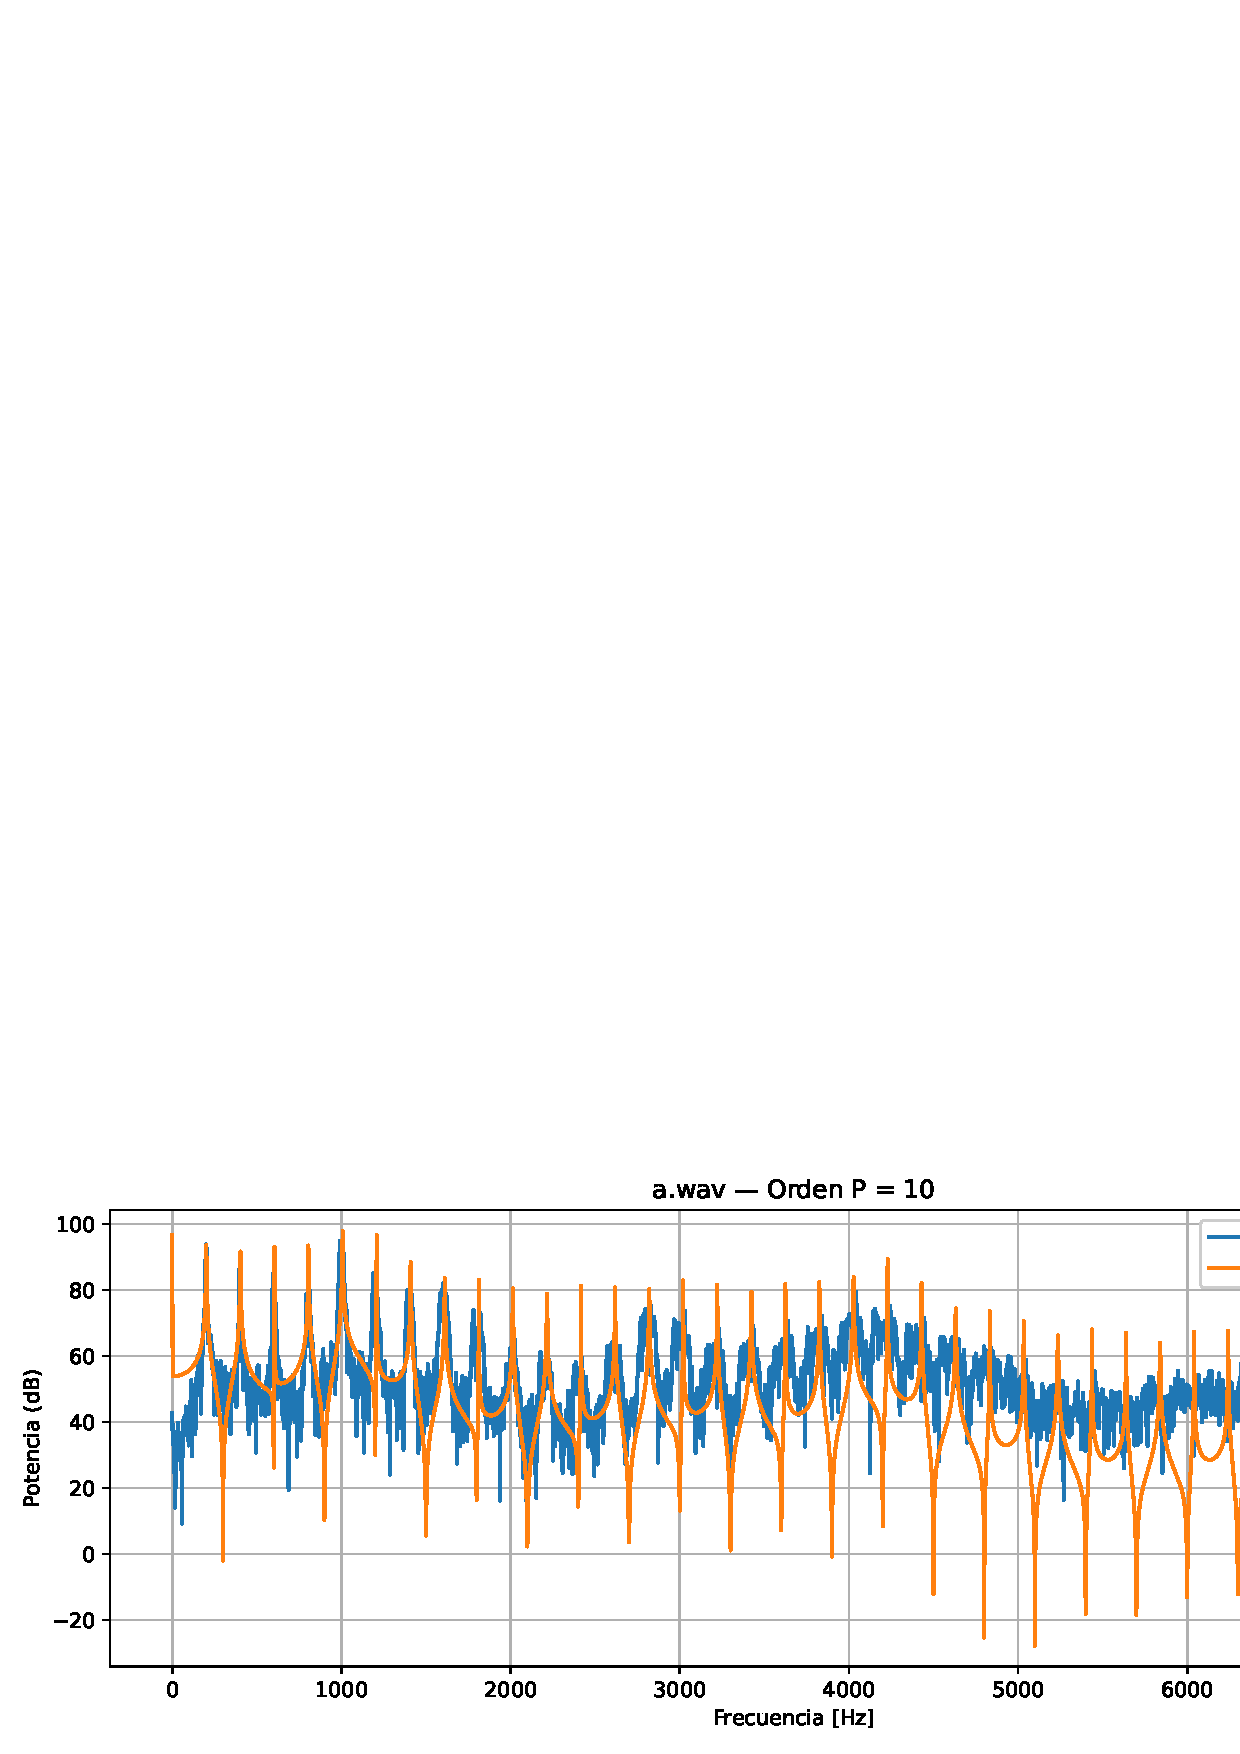
\includegraphics[width=\linewidth]{res/psd_vs_lpc_a_10.pdf}
    \caption{PSD real superpuesta a la obtenida con el modelo de orden 10}
    \label{fig:psd_vs_lpc_a_10}
\end{figure}

\begin{figure}[H]
    \centering
    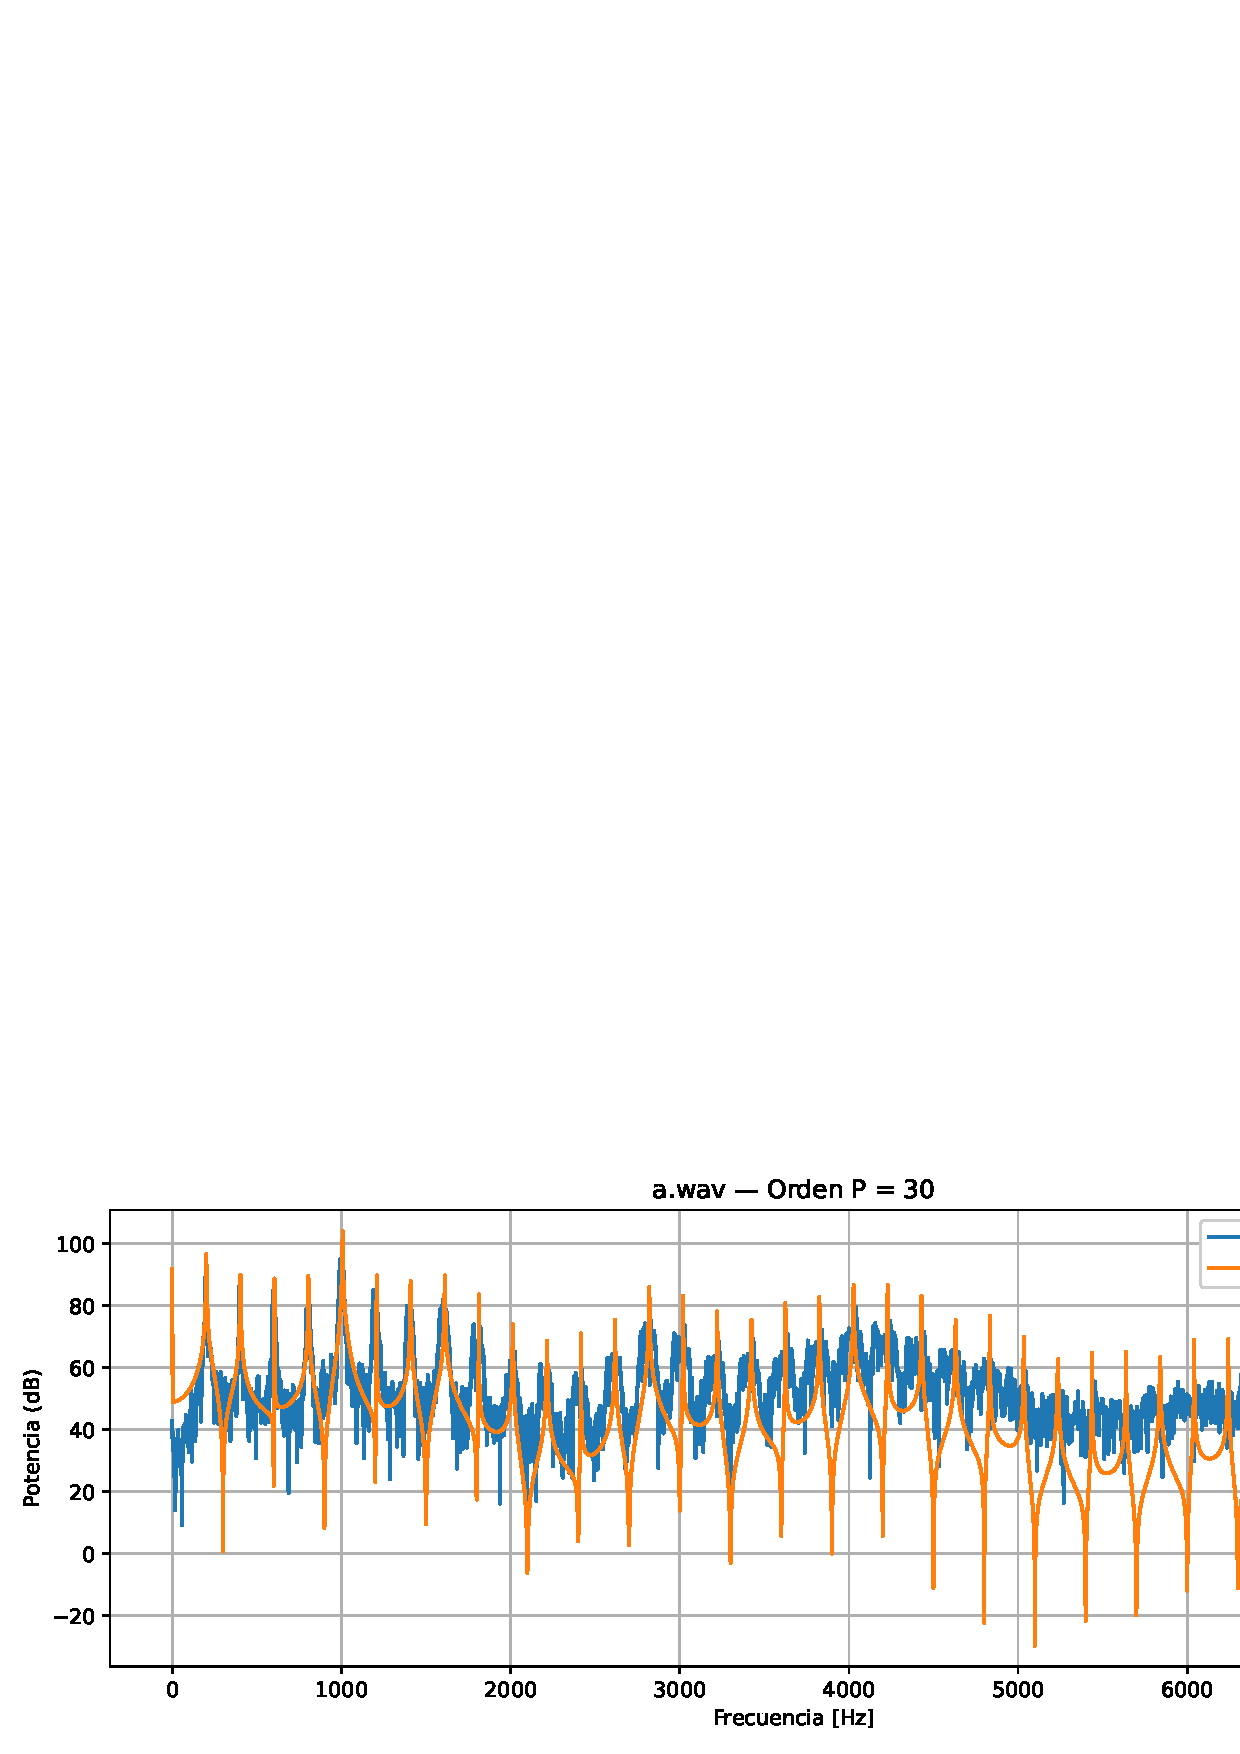
\includegraphics[width=\linewidth]{res/psd_vs_lpc_a_30.pdf}
    \caption{PSD real superpuesta a la obtenida con el modelo de orden 30}
    \label{fig:psd_vs_lpc_a_30}
\end{figure}

\subsection{Sonido ``e''}

\begin{figure}[H]
    \centering
    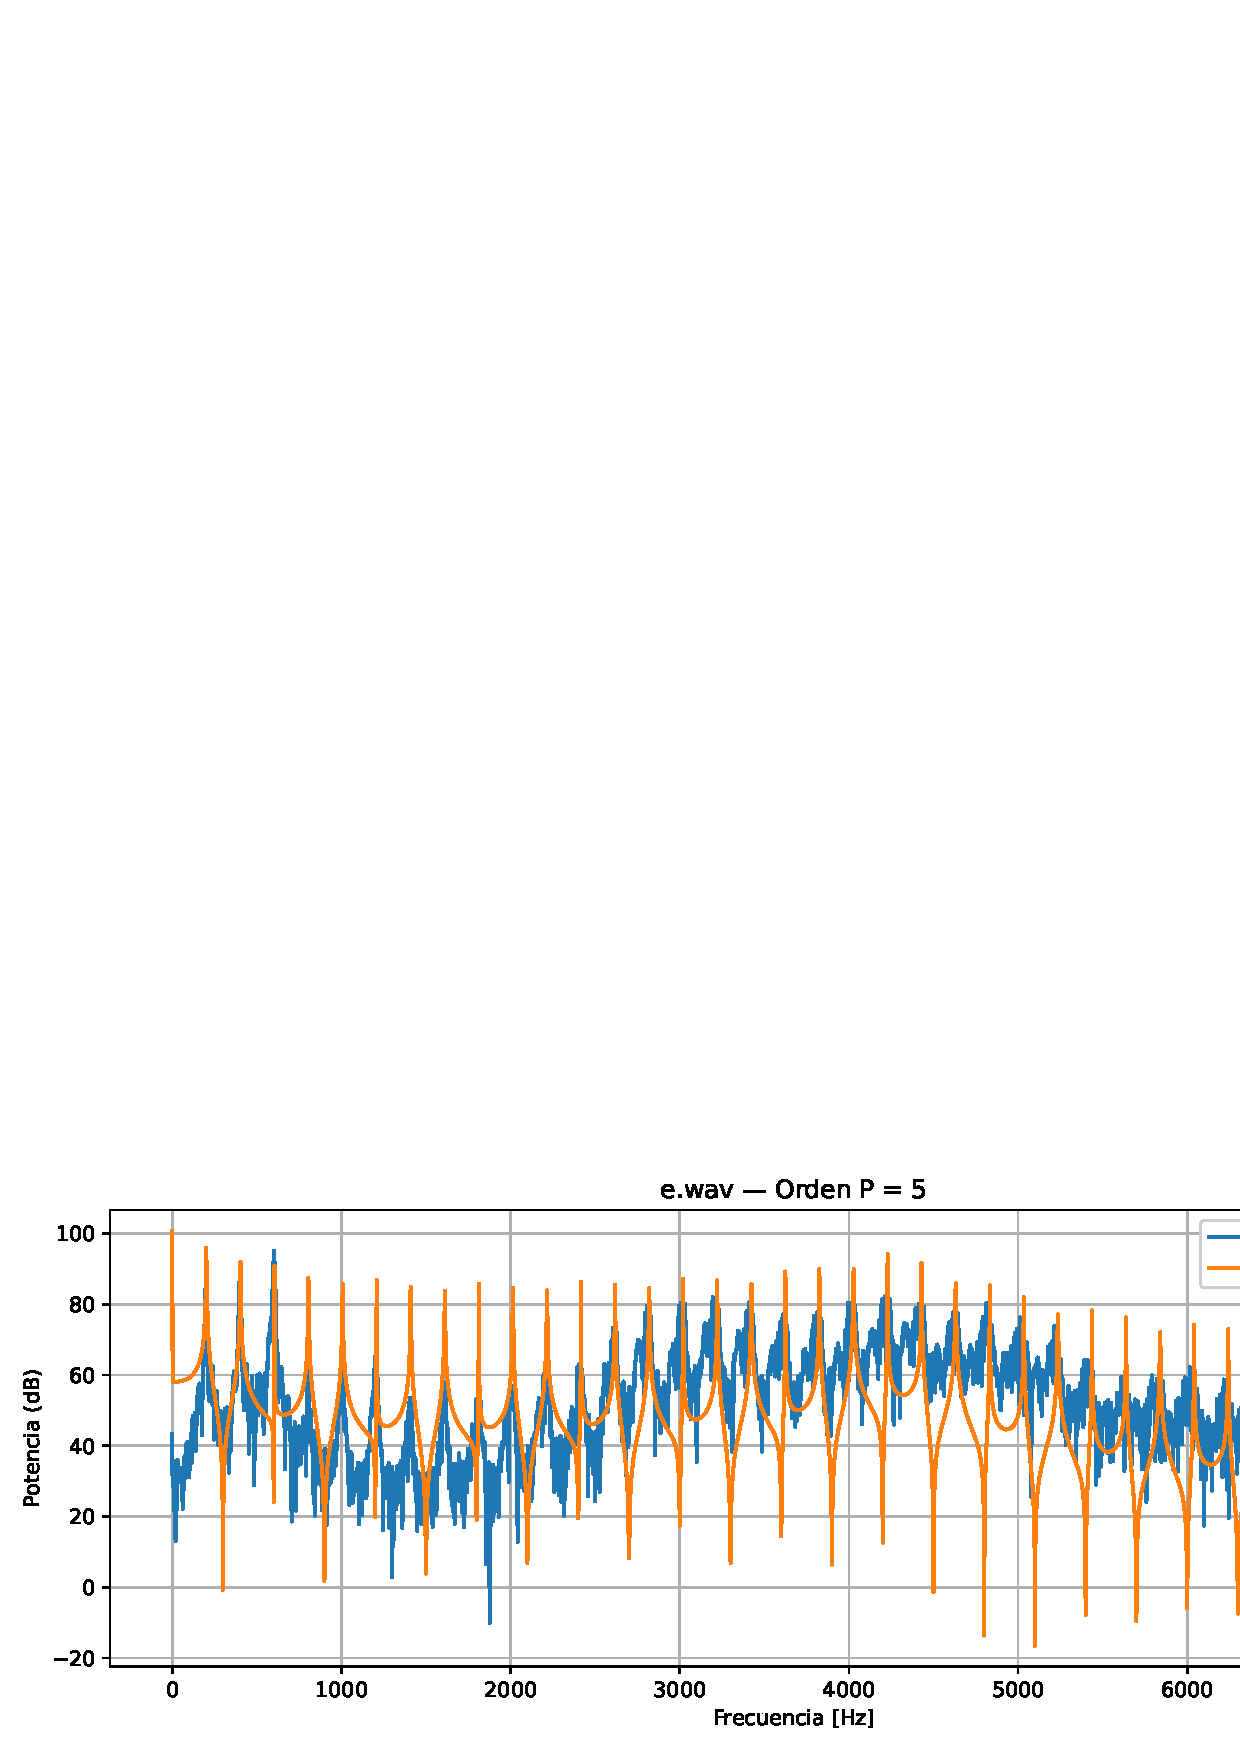
\includegraphics[width=\linewidth]{res/psd_vs_lpc_e_5.pdf}
    \caption{PSD real superpuesta a la obtenida con el modelo de orden 5}
    \label{fig:psd_vs_lpc_e_5}
\end{figure}

\begin{figure}[H]
    \centering
    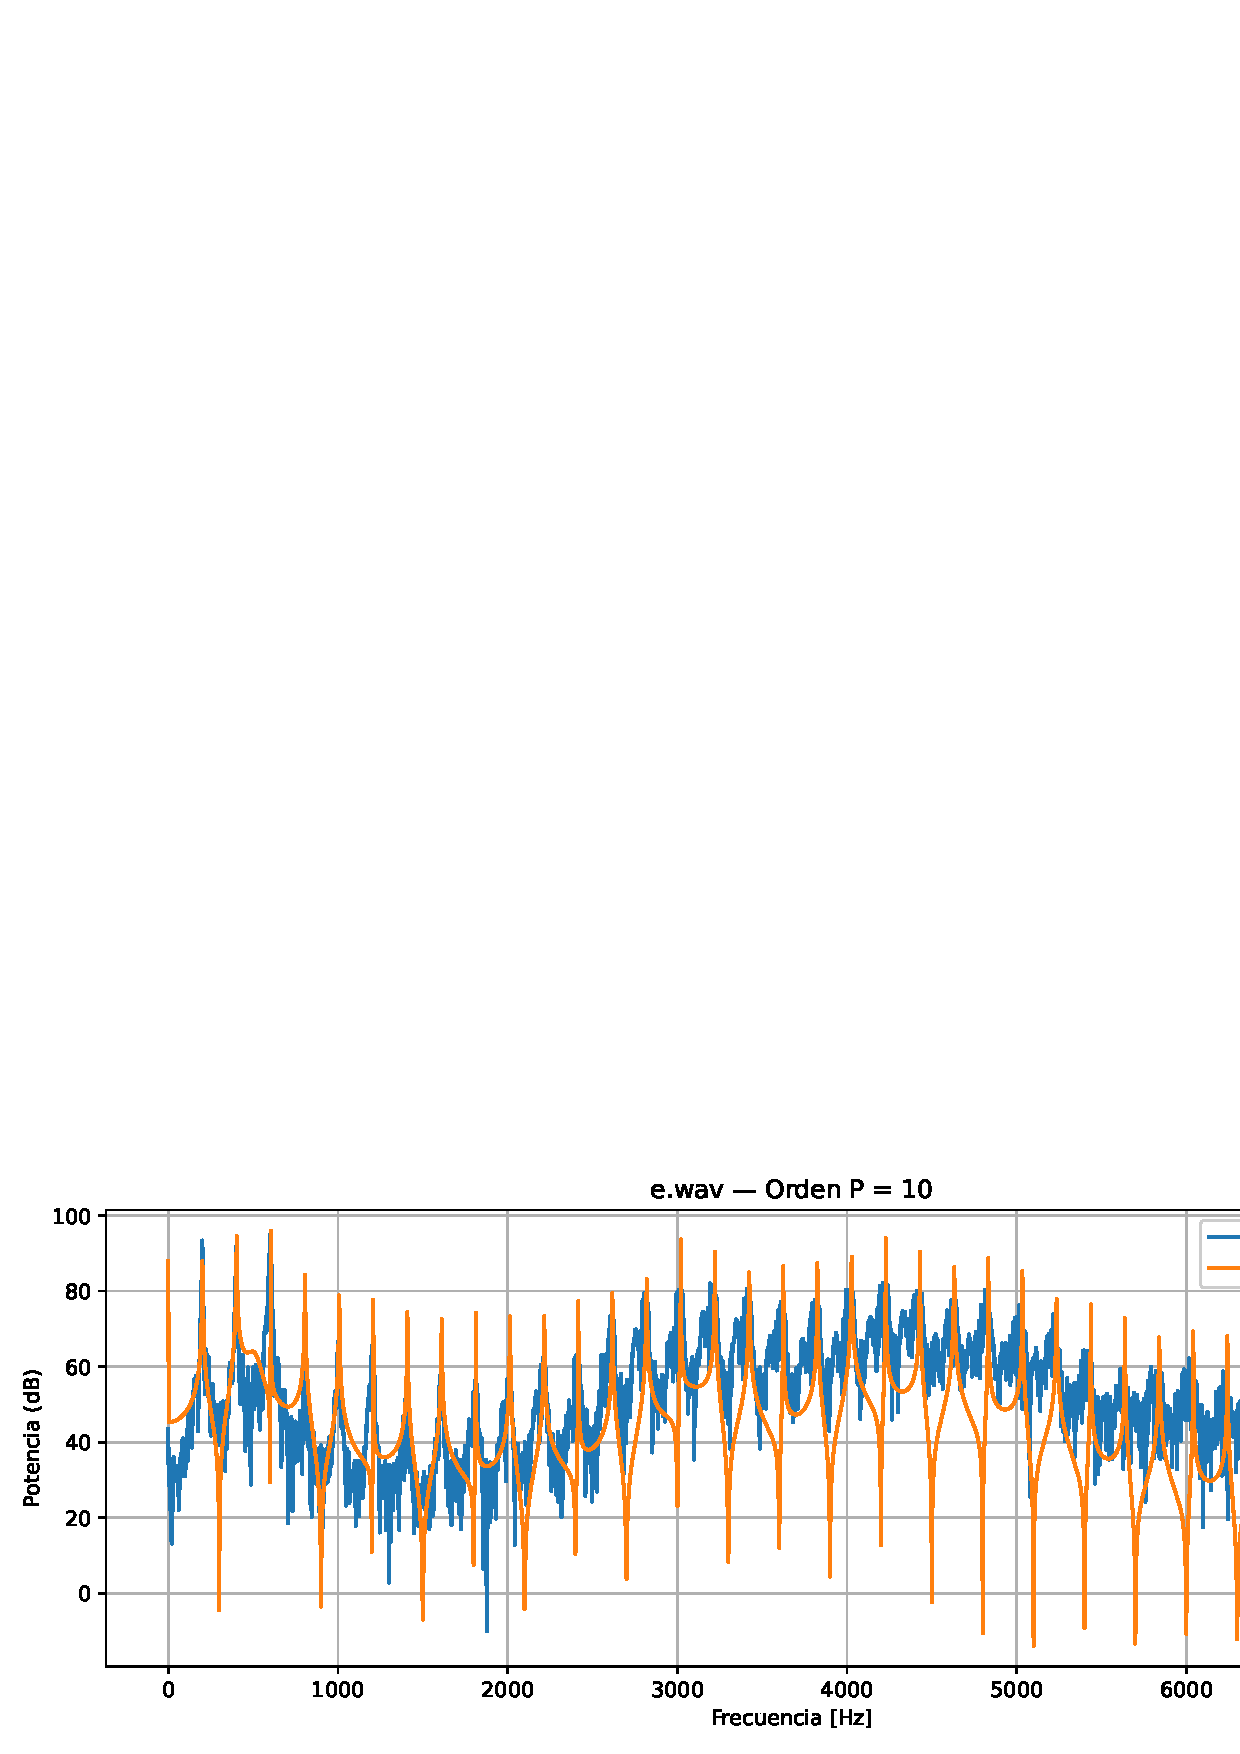
\includegraphics[width=\linewidth]{res/psd_vs_lpc_e_10.pdf}
    \caption{PSD real superpuesta a la obtenida con el modelo de orden 10}
    \label{fig:psd_vs_lpc_e_10}
\end{figure}

\begin{figure}[H]
    \centering
    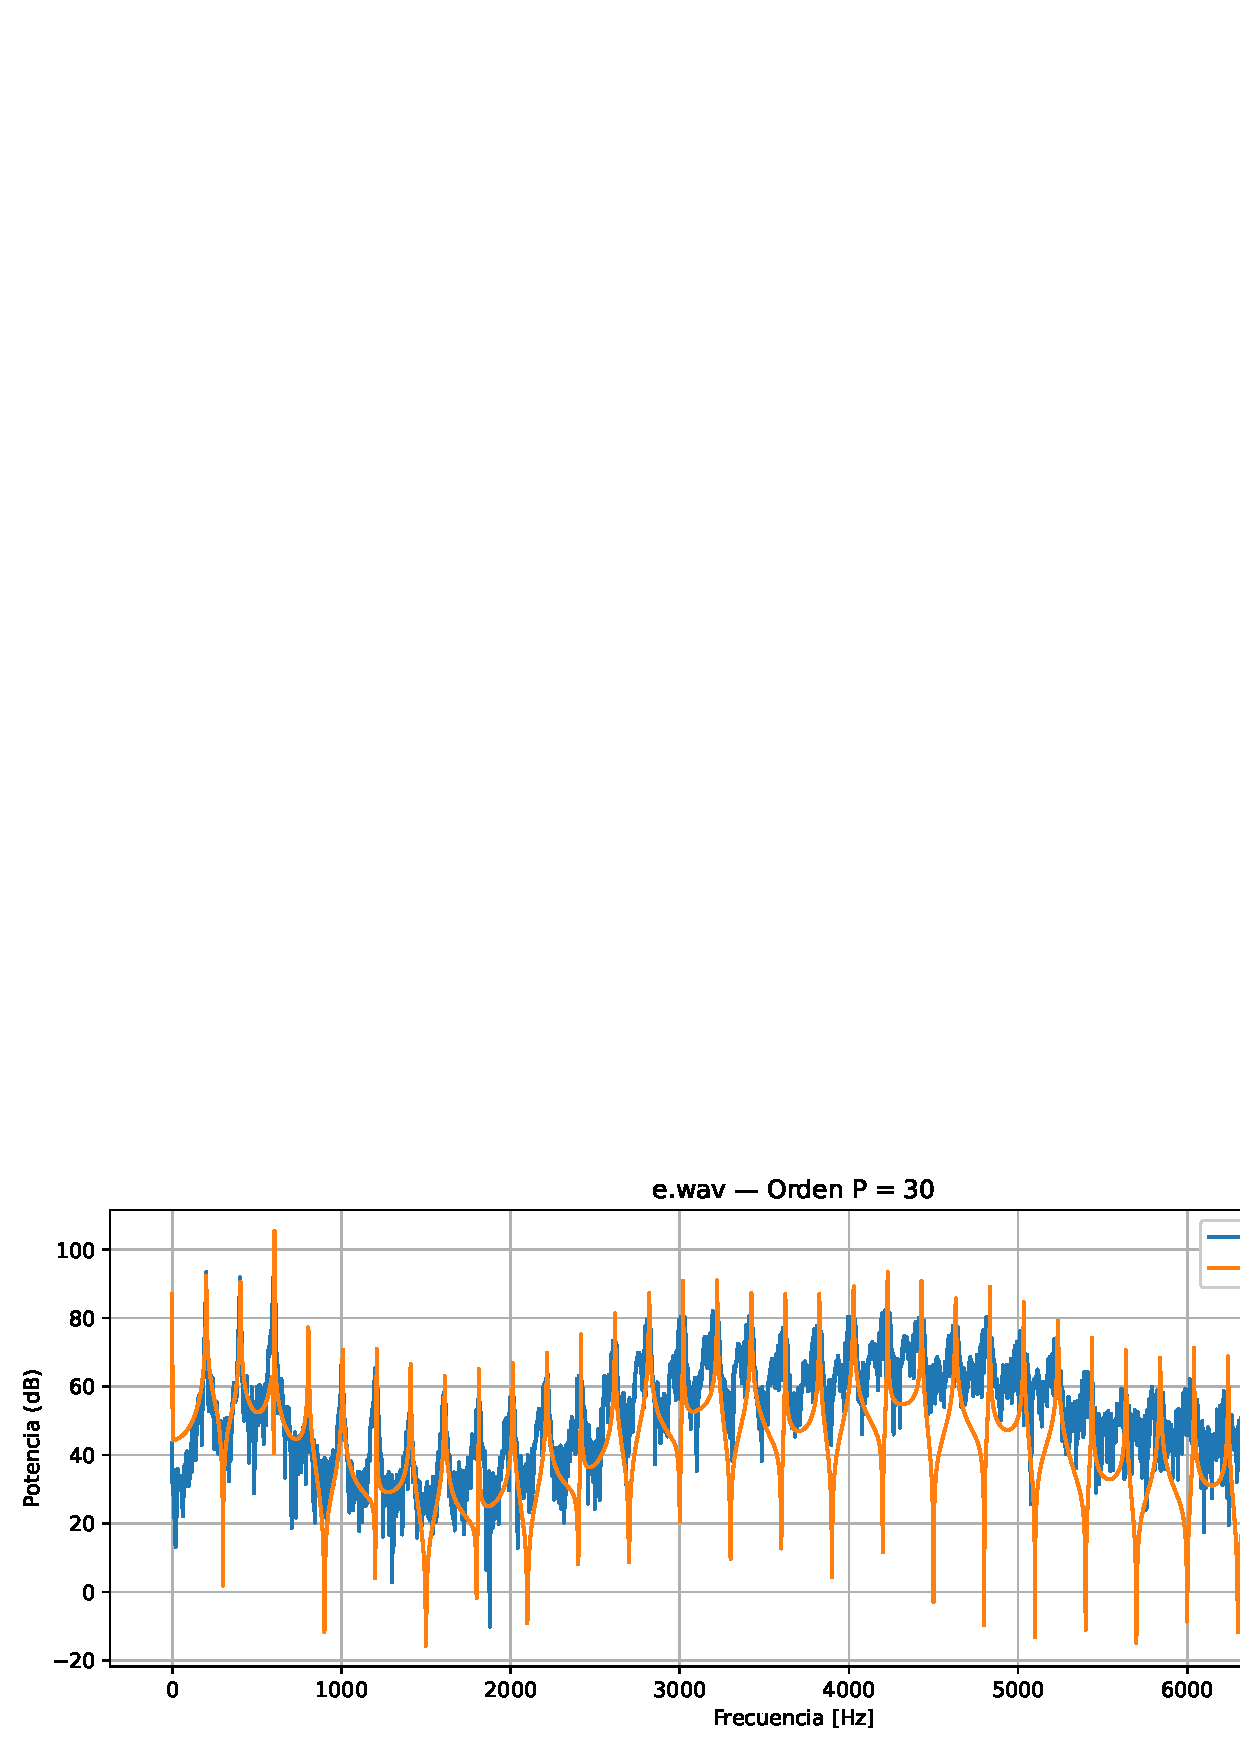
\includegraphics[width=\linewidth]{res/psd_vs_lpc_e_30.pdf}
    \caption{PSD real superpuesta a la obtenida con el modelo de orden 30}
    \label{fig:psd_vs_lpc_e_30}
\end{figure}

\subsection{Sonido ``s''}

\begin{figure}[H]
    \centering
    \includegraphics[width=\linewidth]{res/psd_vs_lpc_s_5.pdf}
    \caption{PSD real superpuesta a la obtenida con el modelo de orden 5}
    \label{fig:psd_vs_lpc_s_5}
\end{figure}

\begin{figure}[H]
    \centering
    \includegraphics[width=\linewidth]{res/psd_vs_lpc_s_10.pdf}
    \caption{PSD real superpuesta a la obtenida con el modelo de orden 10}
    \label{fig:psd_vs_lpc_s_10}
\end{figure}

\begin{figure}[H]
    \centering
    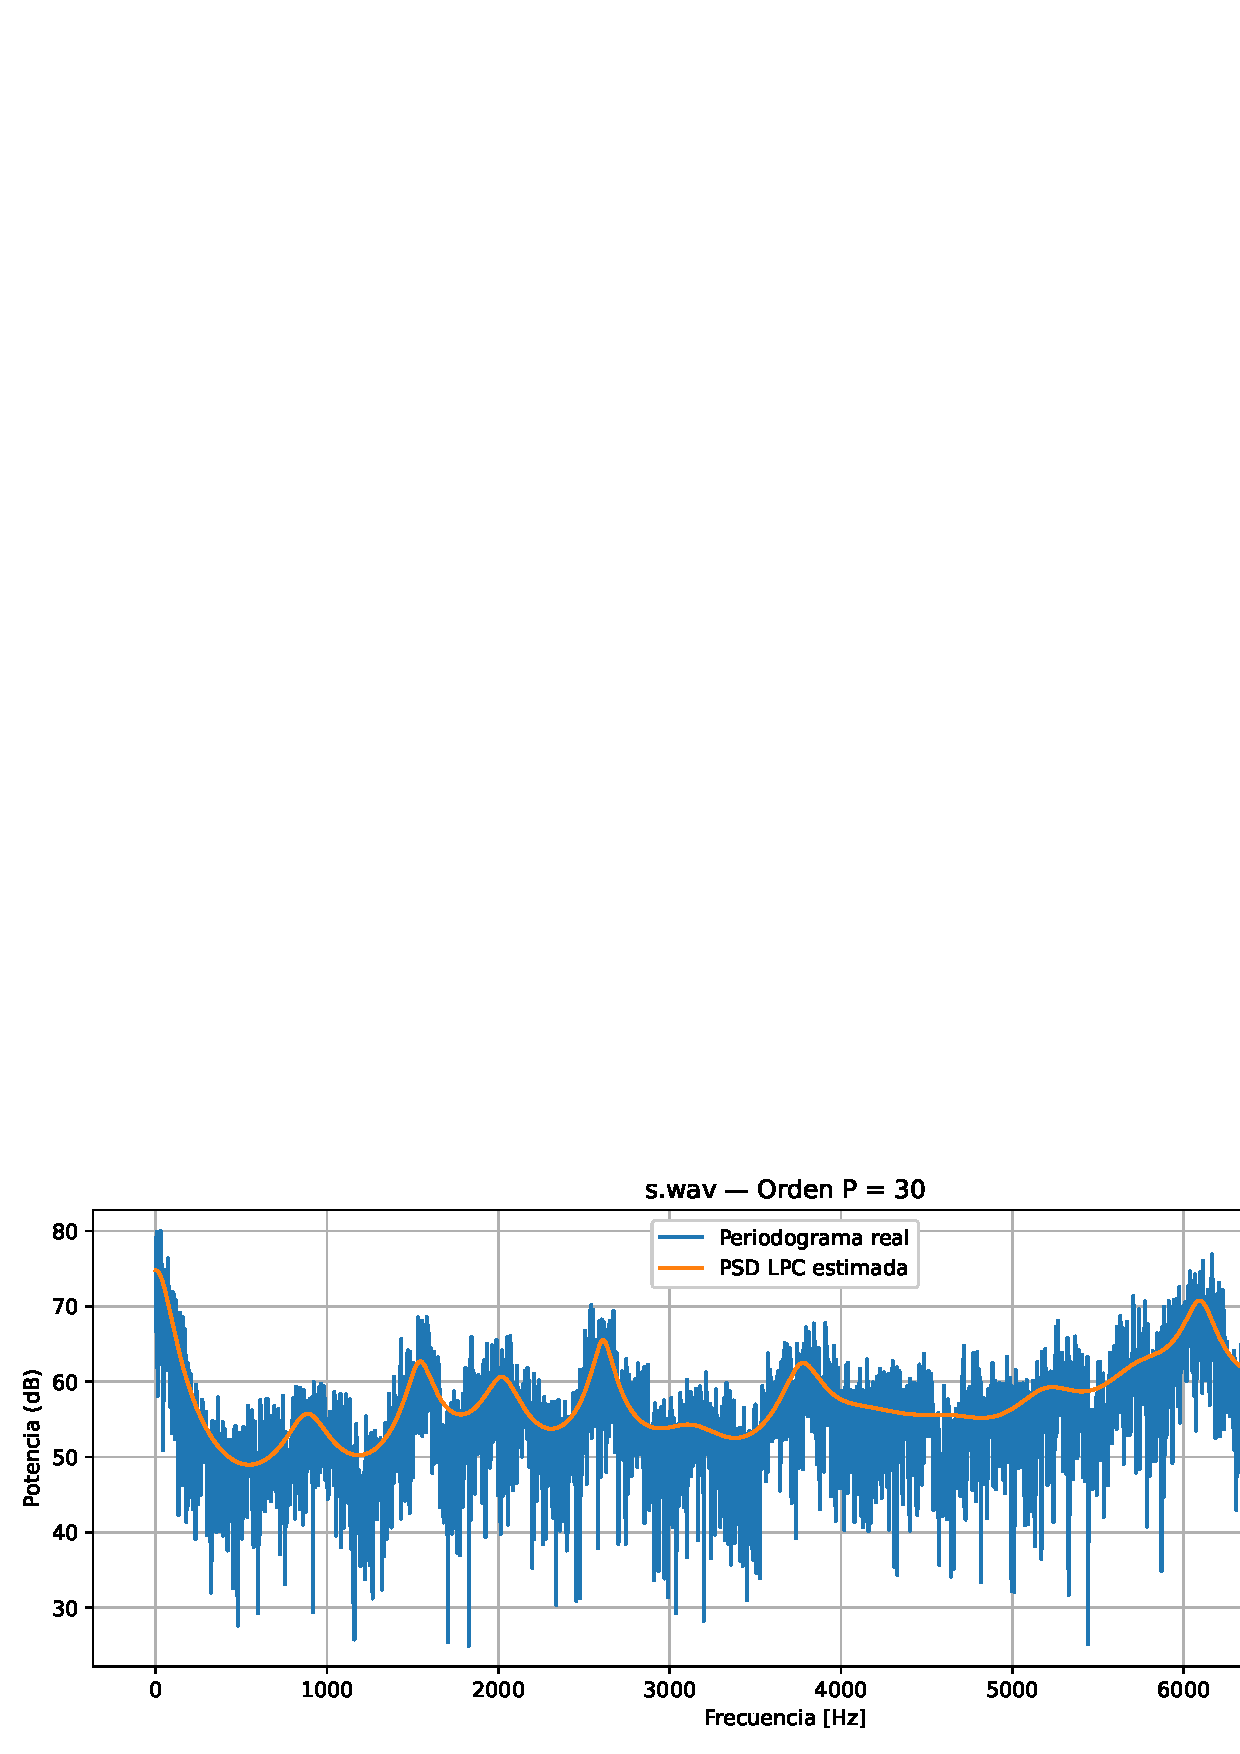
\includegraphics[width=\linewidth]{res/psd_vs_lpc_s_30.pdf}
    \caption{PSD real superpuesta a la obtenida con el modelo de orden 30}
    \label{fig:psd_vs_lpc_s_30}
\end{figure}

\subsection{Sonido ``sh''}

\begin{figure}[H]
    \centering
    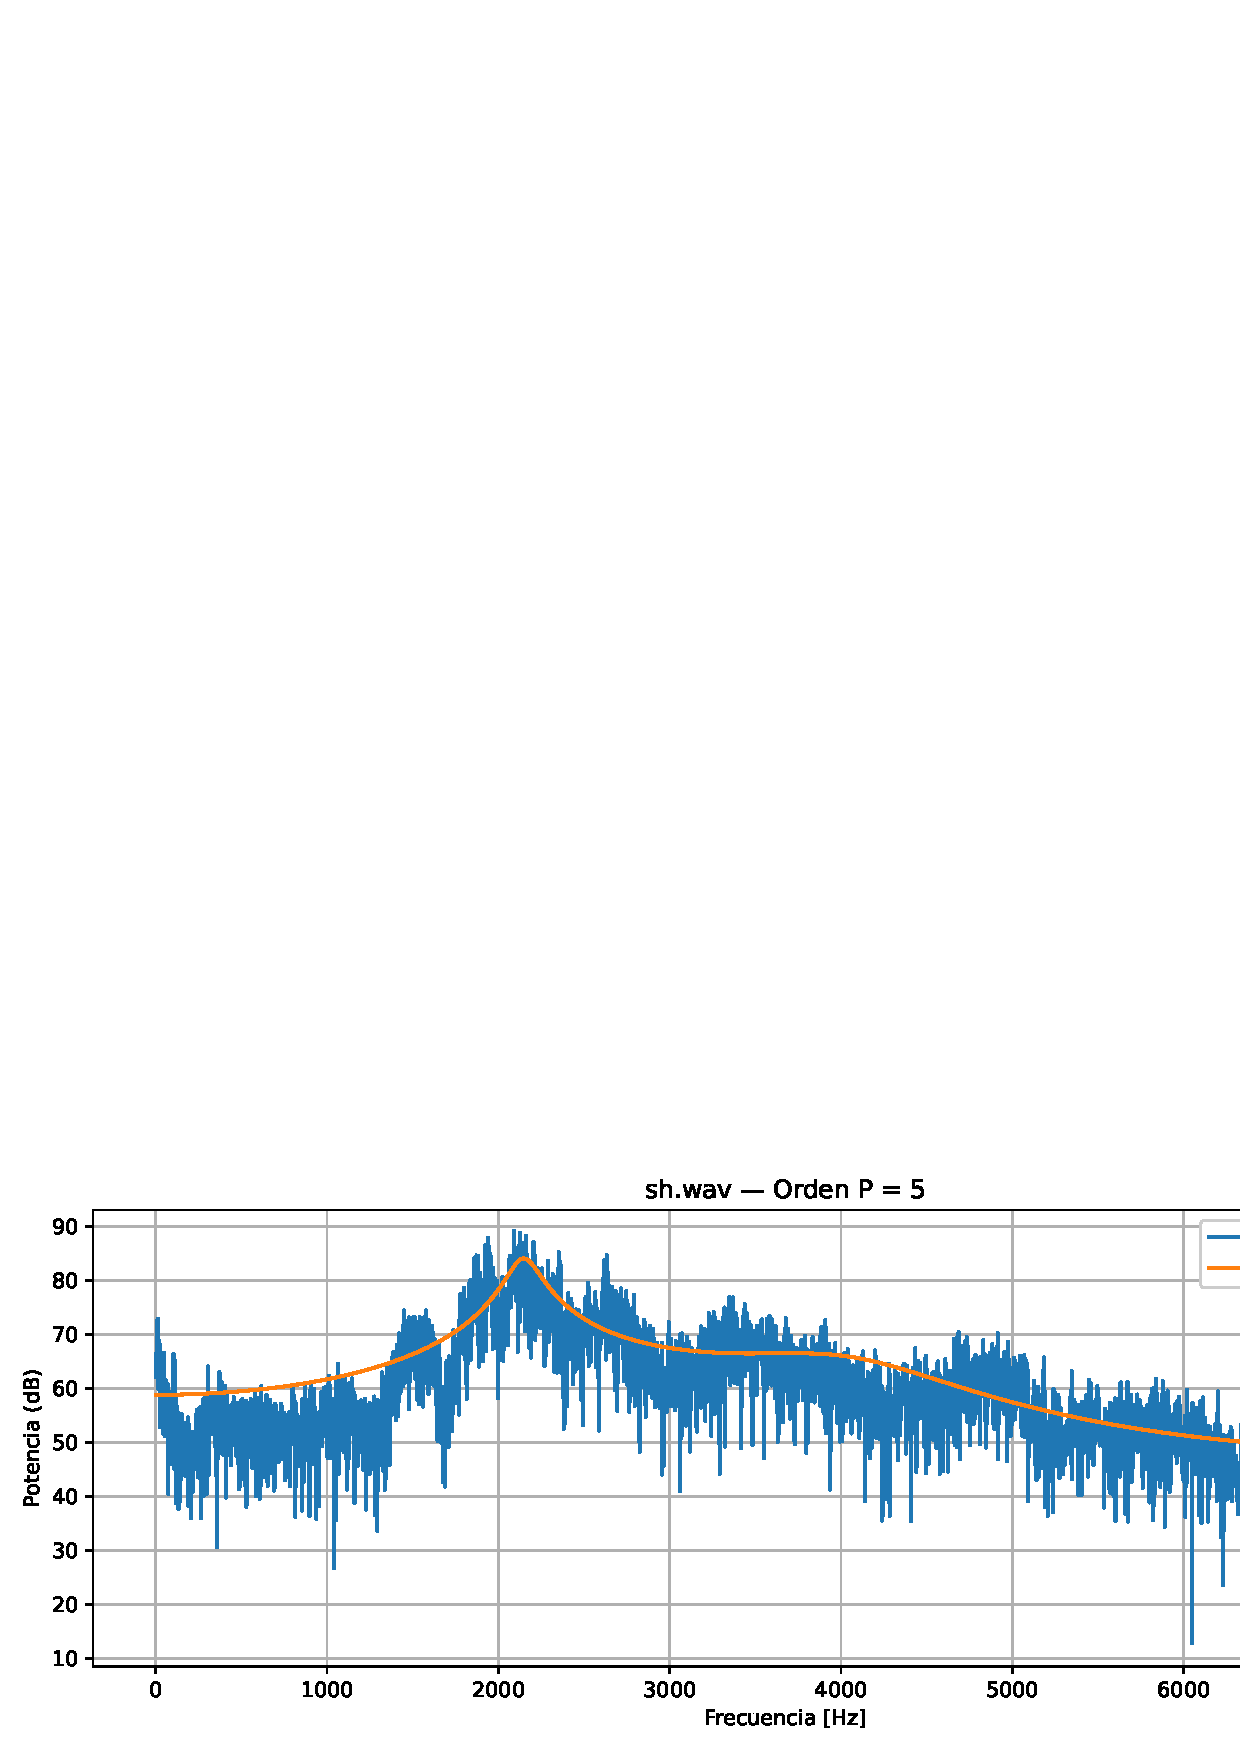
\includegraphics[width=\linewidth]{res/psd_vs_lpc_sh_5.pdf}
    \caption{PSD real superpuesta a la obtenida con el modelo de orden 5}
    \label{fig:psd_vs_lpc_sh_5}
\end{figure}

\begin{figure}[H]
    \centering
    \includegraphics[width=\linewidth]{res/psd_vs_lpc_sh_10.pdf}
    \caption{PSD real superpuesta a la obtenida con el modelo de orden 10}
    \label{fig:psd_vs_lpc_sh_10}
\end{figure}

\begin{figure}[H]
    \centering
    \includegraphics[width=\linewidth]{res/psd_vs_lpc_sh_30.pdf}
    \caption{PSD real superpuesta a la obtenida con el modelo de orden 30}
    \label{fig:psd_vs_lpc_sh_30}
\end{figure}

\subsection{Análisis de resultados}

\quad En el caso de los fonemas sonoros el ajuste es cercano para todos los ordenes, sin embargo se denota una clara mejora al aumentar la cantidad de coeficientes. El ajuste de la ganancia es considerablemente más preciso y el comportamiento fuera de los picos es menos brusco. 

\quad Sin embargo, el efecto de variar el orden tiene mayor peso en los fonemas sordos. En estos se ve claramente como la forma estimada con el orden 5 sigue la forma general de la onda pero no la de sus picos. Al aumentar el orden el seguimiento mejora notablemente, en el orden 30 se ve como la curva se ajusta a los picos principales de la señal ademas de seguir de forma mas fiel la señal general. 

\section{Detección de pitch}

%%%%%Esto se conecta con lo de abajo, no toco los mismos puntos.
\quad Como se mencionó anteriormente, es necesario para la sinterización de los fonemas sonoros, no solo estimar los coeficientes del LPC, sino que también detectar la frecuencia fundamental  con el objetivo de reconstruir el mismo sin perder la entonación del audio original.

\quad Para ello es posible modelar el residuo LPC o la autocorrelacion del error de predicción $R_e(k)$. Se modela este parámetro ya que la señal original de voz incluye una excitación periódica y una resonancia del tracto vocal (los formantes), que crean picos adiciones en el espectro, esto hace que la autocorrelacion de la señal completa tenga varios picos grandes y sea difícil de saber cual corresponde al pitch real, utilizando el residuo LPC es posible eliminar esta resonancia y conservar la periodicidad del sonido.

\quad A continuación se resume los pasos desarrollados para la implementación del detector:

\begin{itemize}
    \item Calculo de la señal de error: Se calcula el error de predicción computando \ref{error_de_prediccion}
    \item Autocorrelación de la señal de error: Se calcula la autocorrelación del error y se normaliza con su valor $R_e(0)$ para independizarlo de su amplitud.
    \item Detección de picos: Se implementa una función que busca el segundo pico significativo en la autocorrelacion dentro de un rango. utilizando un umbral $\alpha$ y calculando la frecuencia en la que se encuentra mediante \ref{frecuencia_de_pitch}
\end{itemize}
%%%%%%%%%%%%%%%%

\quad Al momento de realizar la detección de la frecuencia del pitch se investigo el rango de frecuencias de la voz humana. Se limito la búsqueda a ese rango para disminuir la complejidad computacional del problema y evitar picos espurios. El rango de frecuencias considerado fue $[80Hz, 400Hz]$. 

\quad El valor de $\alpha$ fue elegido observando el gráfico de la auto-correlación del error de las vocales. En ambos se puede observar que el valor del segundo pico es siempre mayor a 0.4, por lo tanto se elige un valor apenas menor para tener un margen de error y una seguridad para el resto de las vocales. Teniendo en cuenta todas estas consideraciones se eligió usar $\alpha = 0.4$.

\quad El orden elegido para el LPC fue P = 20. Se considero que sea suficiente para poder diferenciar de manera clara los picos y donde ya no se perciba una diferencia notable al aumentarlo, ya que esto elevaría la complejidad del problema sin presentar un beneficio perceptible. 

\begin{figure}[H]
    \centering
    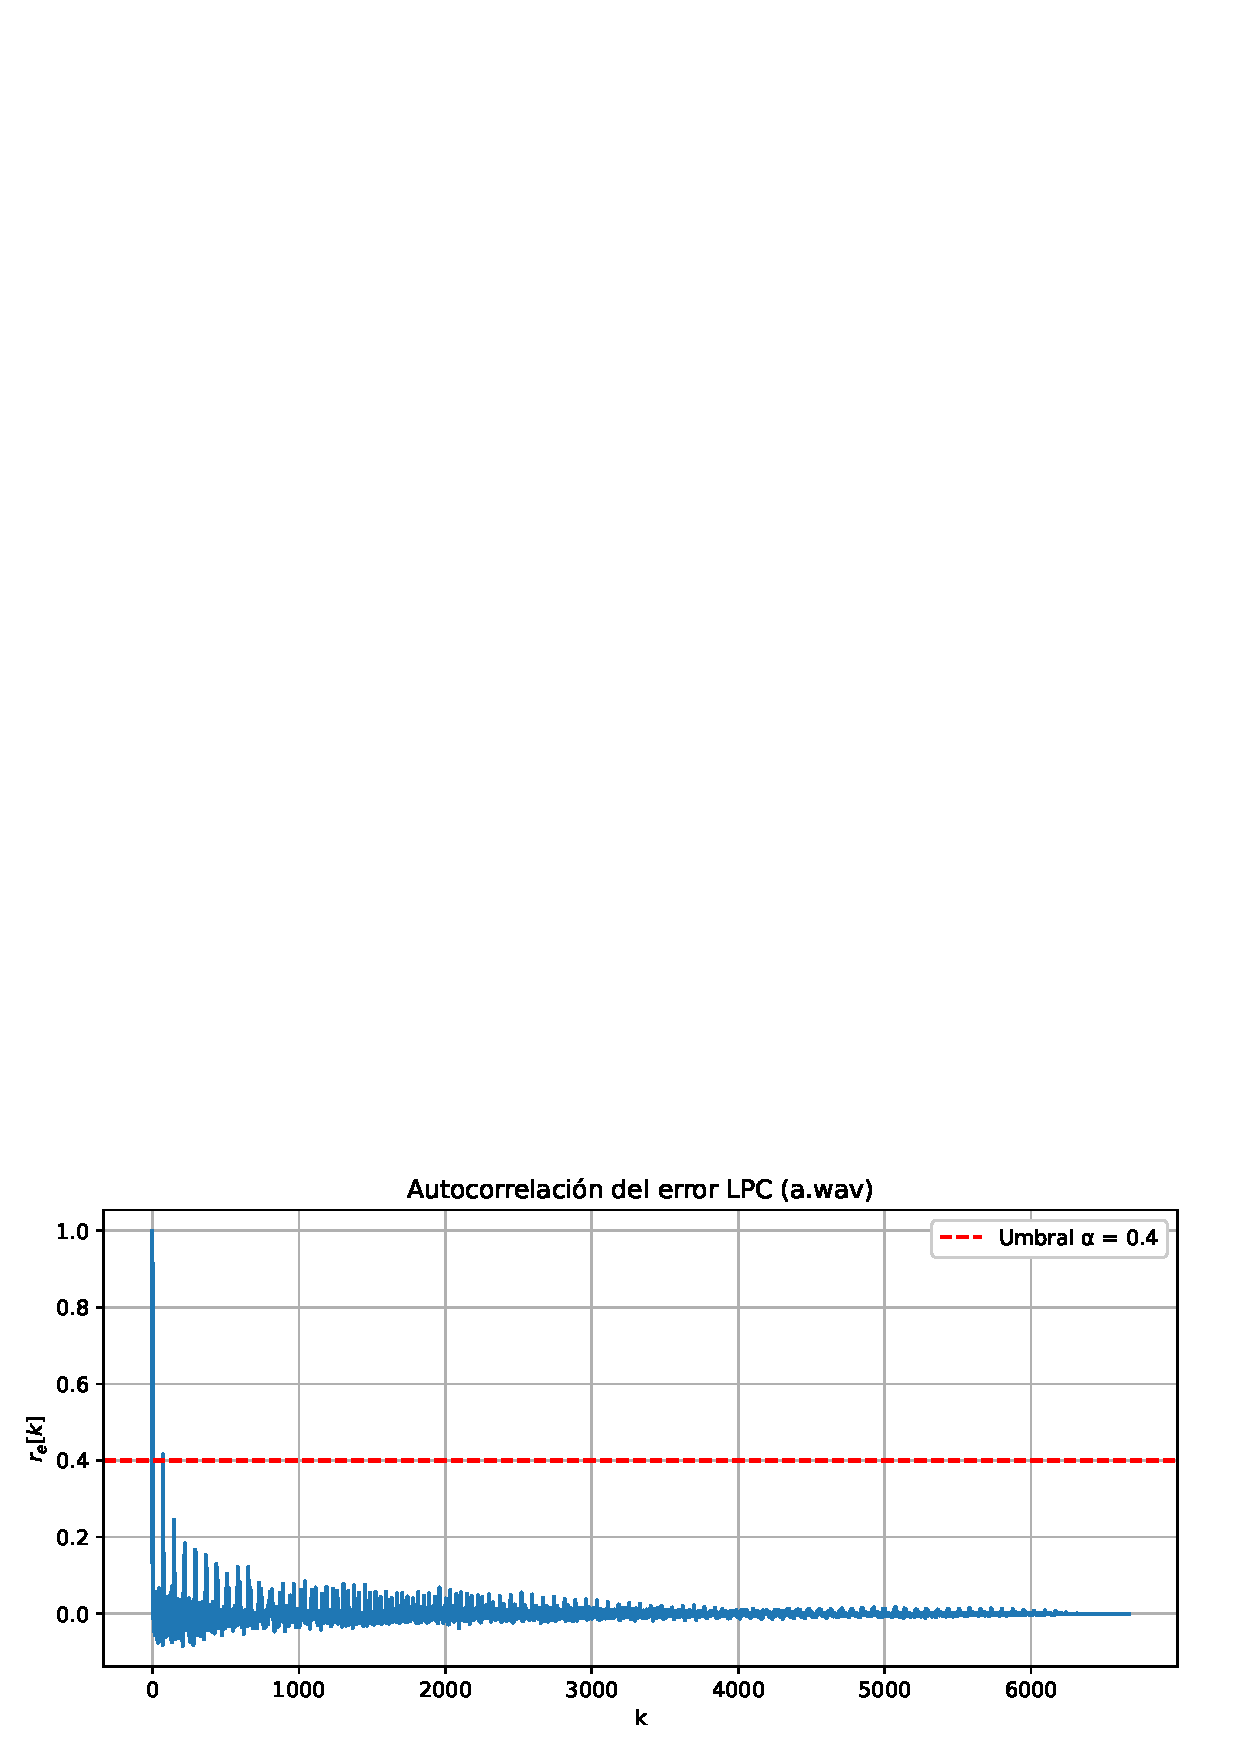
\includegraphics[width=\linewidth]{res/pitch_lpc_a.pdf}
    \caption{Detección de pitch con autocorrelacion de fonema ``a''}
    \label{fig:pitch_lpc_a}
\end{figure}

\begin{figure}
    \centering
    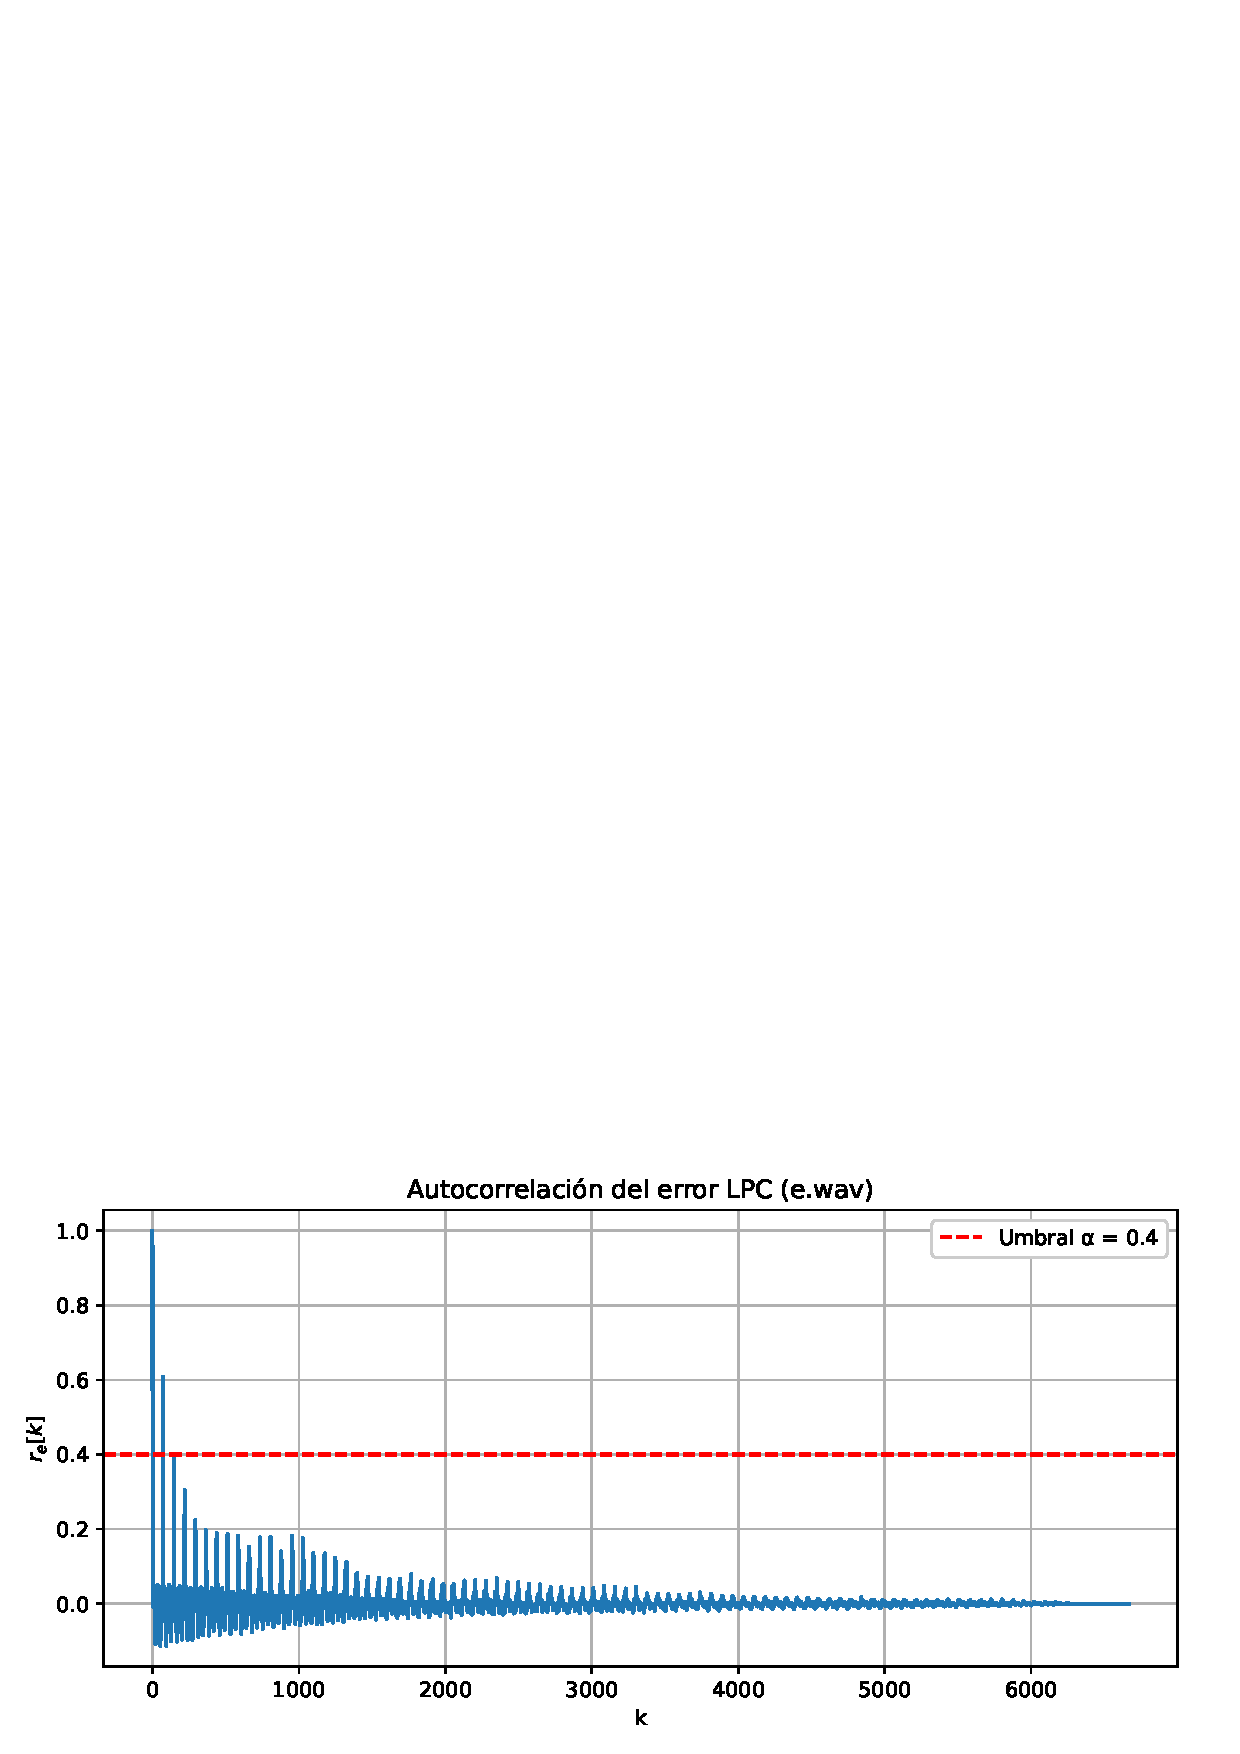
\includegraphics[width=\linewidth]{res/pitch_lpc_e.pdf}
    \caption{Detección de pitch con autocorrelacion de fonema ``e''}
    \label{fig:pitch_lpc_e}
\end{figure}

\begin{figure}[H]
    \centering
    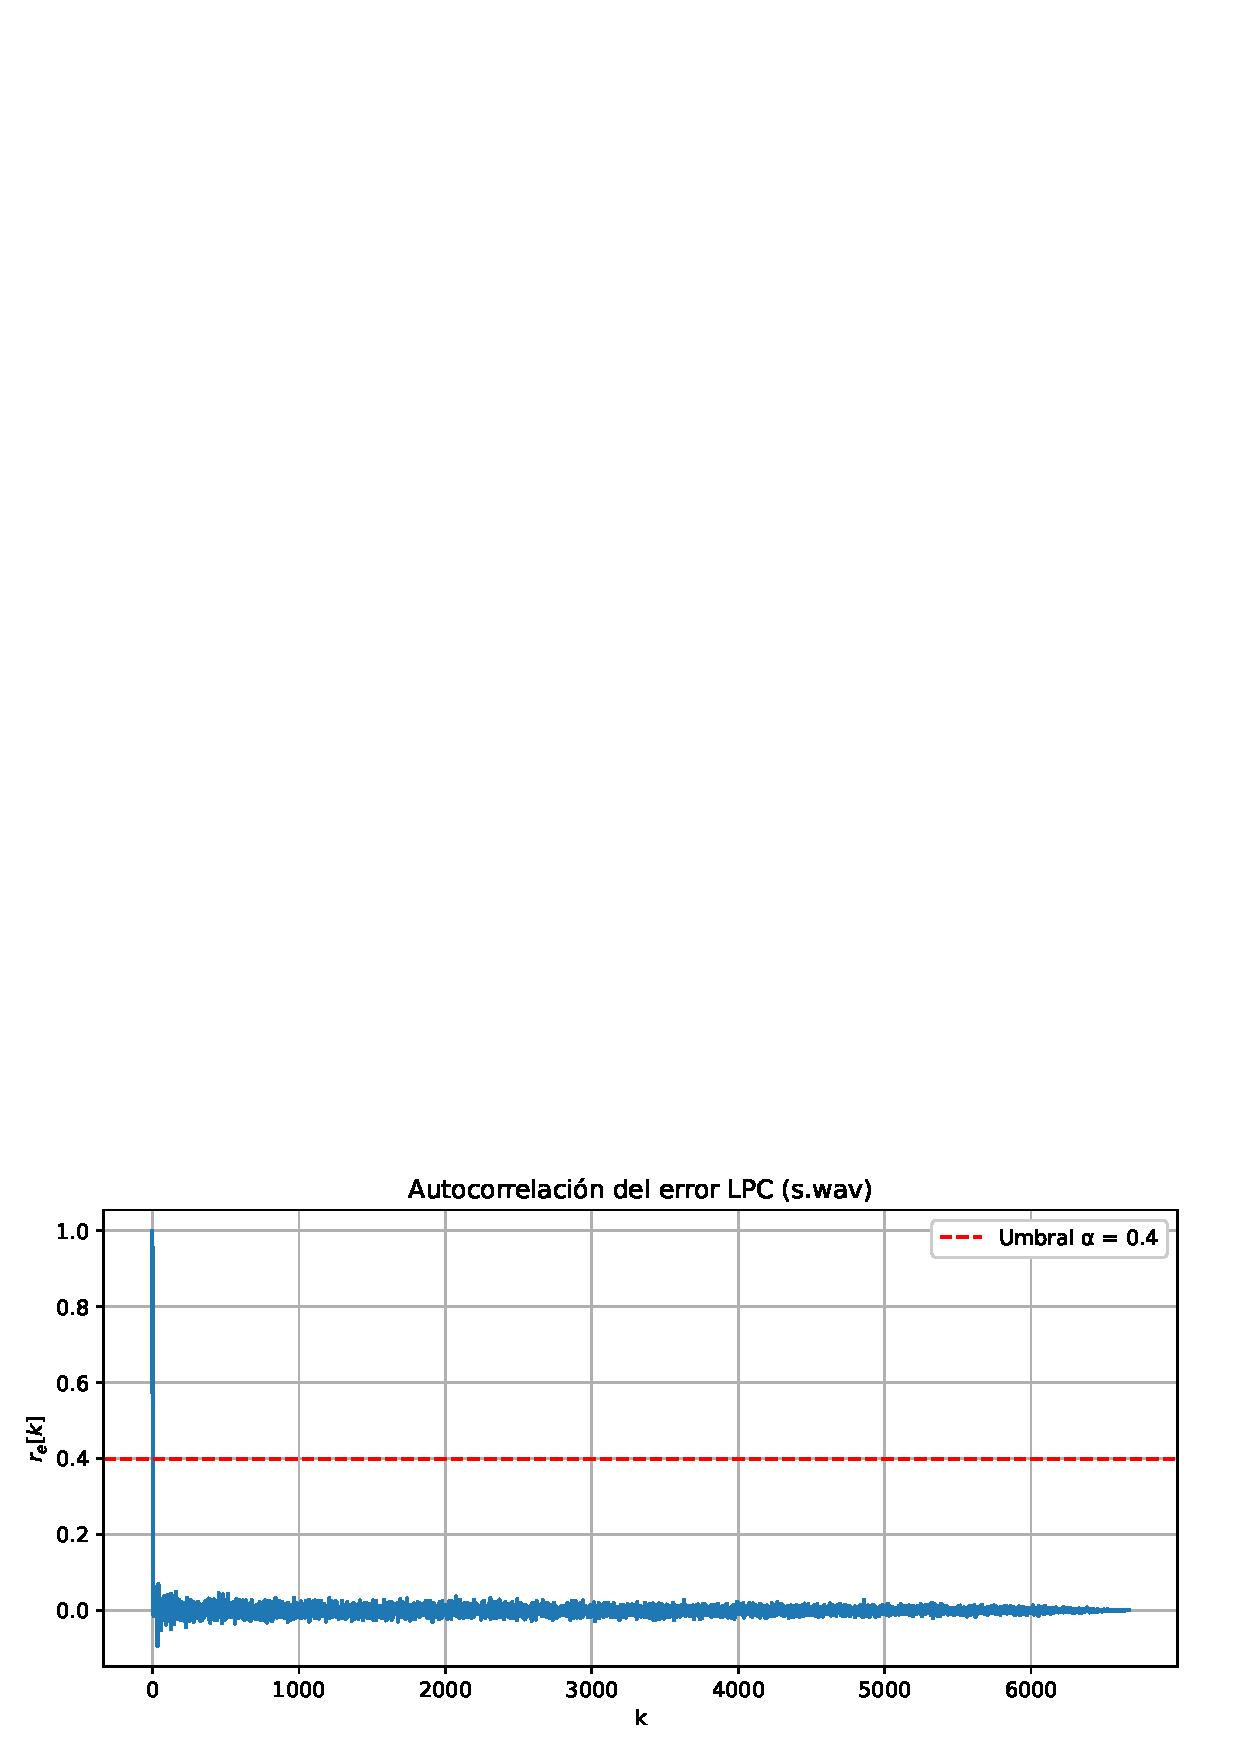
\includegraphics[width=\linewidth]{res/pitch_lpc_s.pdf}
    \caption{Detección de pitch con autocorrelacion de fonema ``s''}
    \label{fig:pitch_lpc_s}
\end{figure}

\begin{figure}[H]
    \centering
    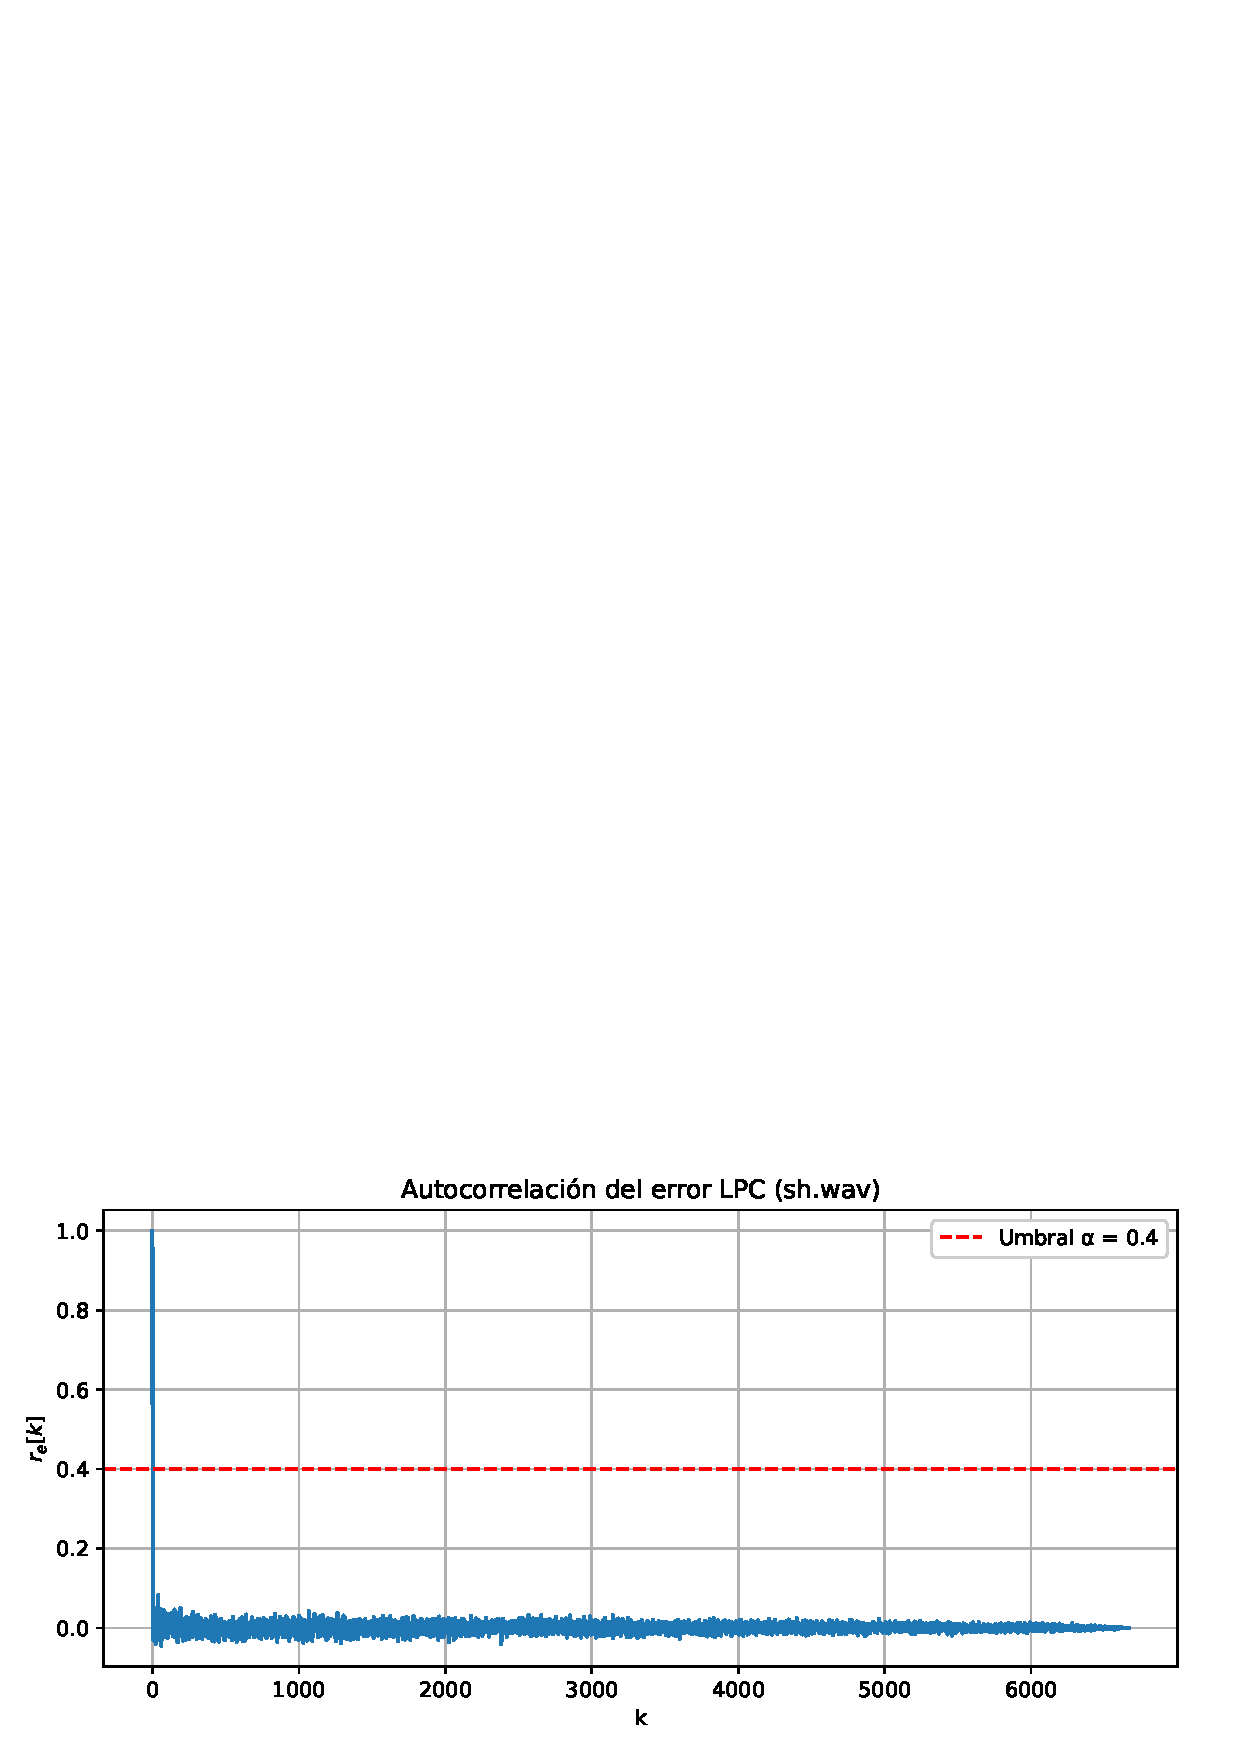
\includegraphics[width=\linewidth]{res/pitch_lpc_sh.pdf}
    \caption{Detección de pitch con autocorrelacion de fonema ``sh''}
    \label{fig:pitch_lpc_sh}
\end{figure}

\quad En las Figuras \ref{fig:pitch_lpc_a}, \ref{fig:pitch_lpc_e}, \ref{fig:pitch_lpc_s} y \ref{fig:pitch_lpc_sh} se puede apreciar como en las vocales el segundo pico supera el umbral elegido y en los fonemas sordos se observa un ruido blanco. Además se observa el valor de los segundos picos en las vocales que fue usado como criterio para elegir donde se ubicó el umbral. 

\subsection{Estimación de PSD con pitch detectado}

\begin{figure}[H]
    \centering
    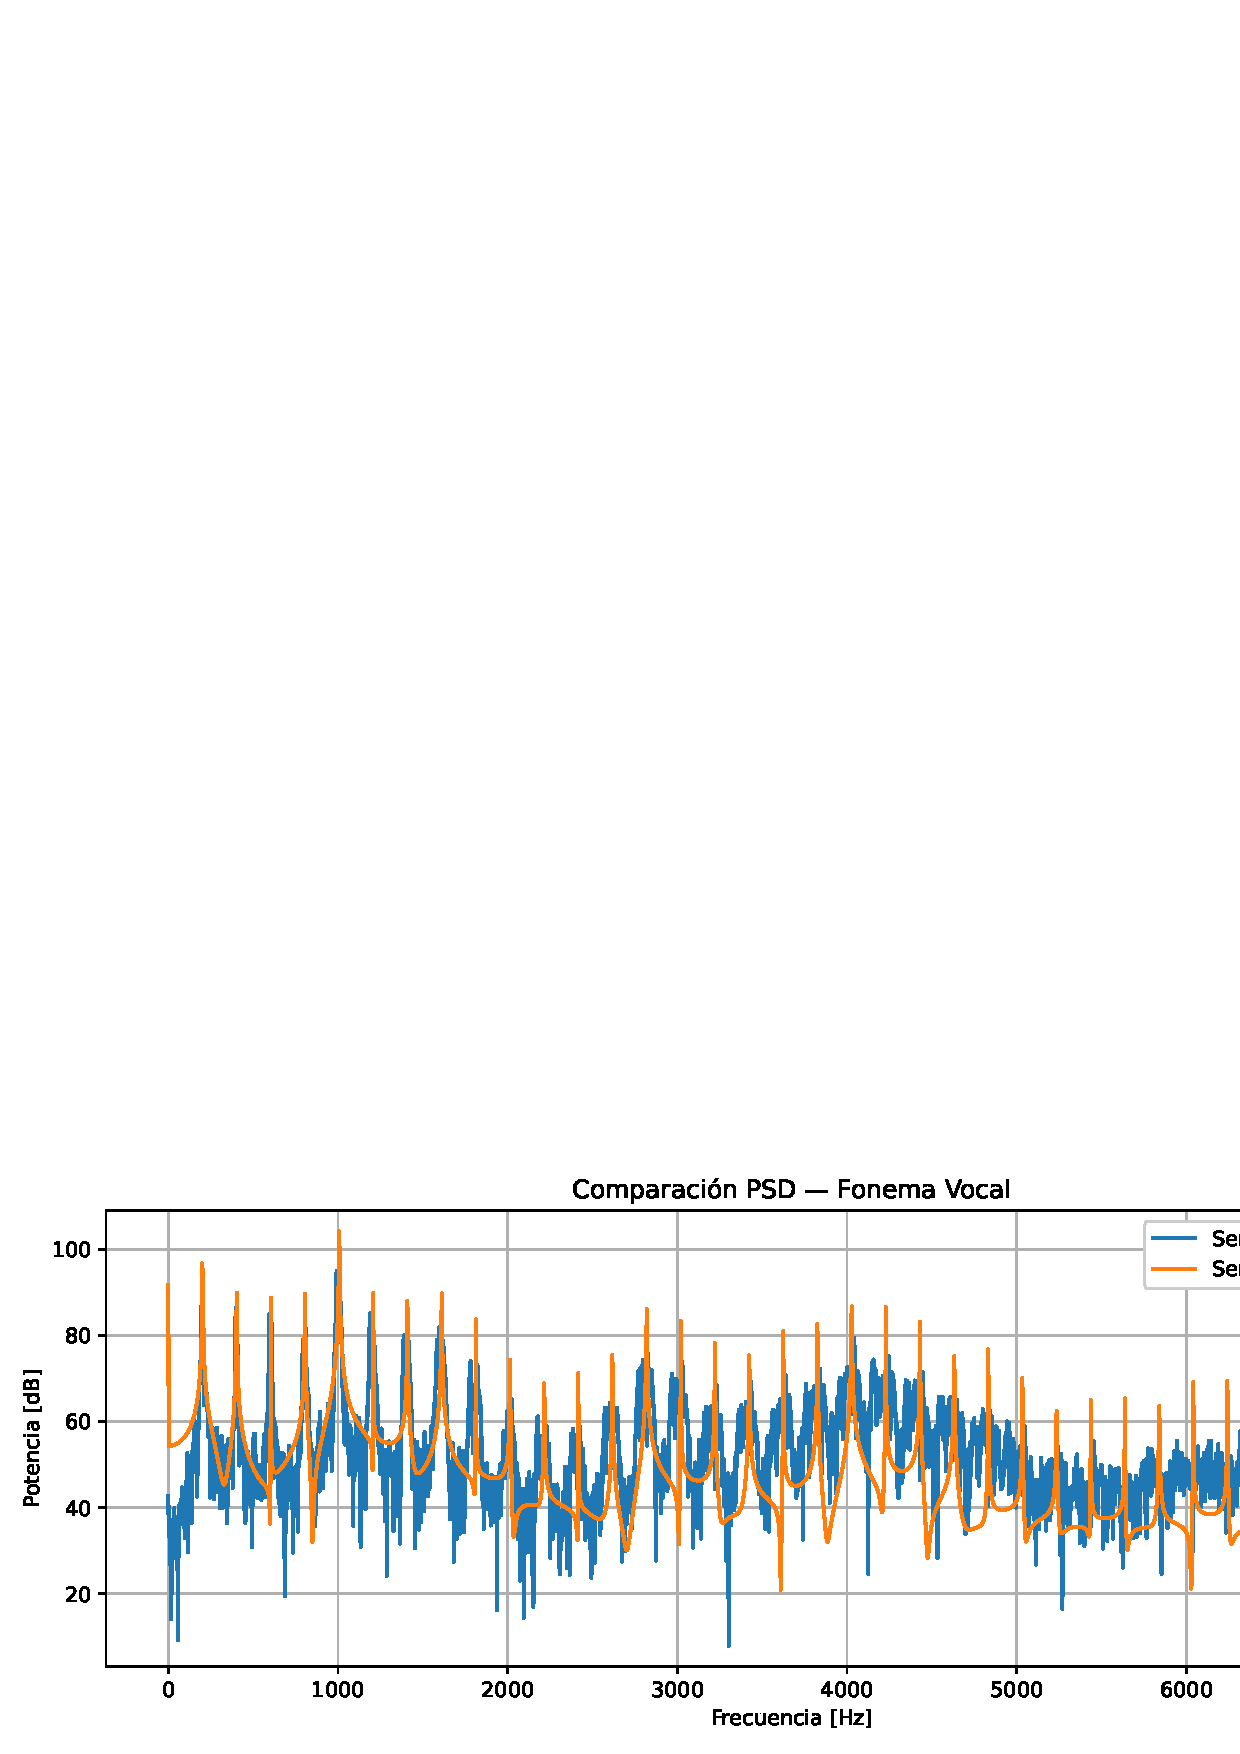
\includegraphics[width=\linewidth]{res/psd_vs_lpc_pitch_a.pdf}
    \caption{PSD obtenida con el pitch detectado}
    \label{fig:psd_vs_lpc_pitch_a}
\end{figure}

\begin{figure}[H]
    \centering
    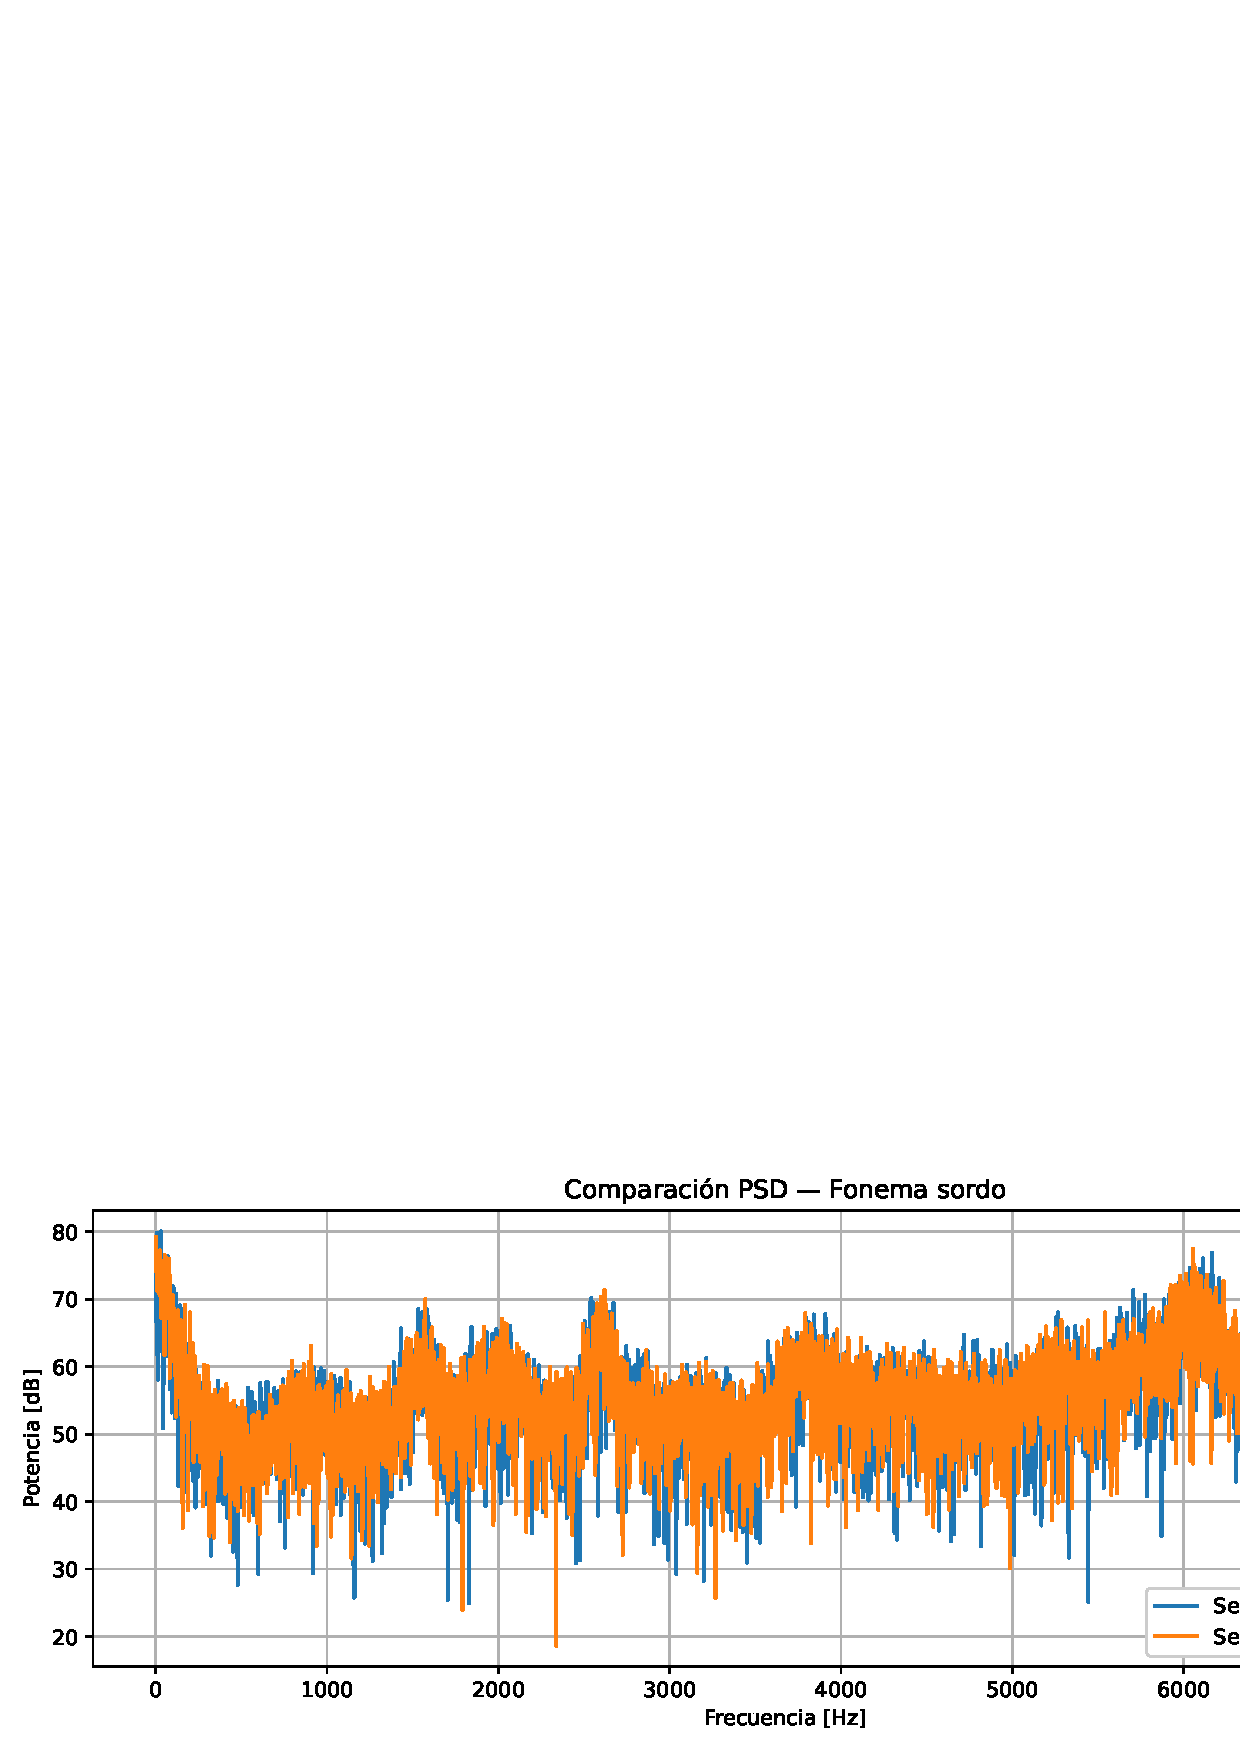
\includegraphics[width=\linewidth]{res/psd_vs_lpc_pitch_s.pdf}
    \caption{PSD de fonema no vocal}
    \label{fig:psd_vs_lpc_pitch_s}
\end{figure}

\quad La frecuencia obtenida con la función \textit{pitch\_lpc} fue de 201.37Hz para ambas vocales, y como se esperaba 0Hz para los fonemas sordos. La frecuencia obtenida es cercana a la usada anteriormente, por lo que se puede ver que la estimación ajusta también de buena forma a la señal real.


\section{Codificación y decodificación}
%%%%%%%intro
    A partir de las pruebas realizadas anteriormente para el correcto funcionamiento la implementación del detector de pitch y estimador de modelo LPC, se procede a realizar una implementación de una codificación y decodificación completa a partir de audios mas extensos provistos por la cátedra.
%%%%%%%

\quad Al momento de codificar el audio se debió considerar que el mismo no es un proceso estacionario. Sin embargo, para poder trabajarlo como si lo fuera se segmento la señal en pequeños fragmentos en donde puedan ser considerados estacionarios y de esa manera usar las simplificaciones de un proceso estacionario. 

%%%%%%%pseudocodigo
    Teniendo esto en cuenta se resume la implementación de la codificación:
    
    \begin{itemize}
        \item Segmentación: La señal de voz se divide en segmentos cortos solapados en una duración de unos pocos milisegundos. La duración de cada segmento debe considerar el compromiso de mantenerse corto para la valides de la cuasi-estacionariedad, y lo suficientemente largo para capturar varios ciclos del tono fundamental respectivo.
        \item Ventaneo: Se opta por multiplicar cada segmento por una ventana de Hamming por sugerencia de la cátedra.
        \item Extracción de parámetros LPC: A cada segmento ventaneado se le extraen los coeficientes y ganancia para el modelo LPC y el pitch respecto en caso de ser detectado como sonoro
    \end{itemize}

Un receptor que quiera reconstruir la señal puede utilizar el siguiente algoritmo implementado para la decodificación:

\begin{itemize}
    \item Síntesis iterativa de segmentos: La función de síntesis procesa cada conjunto de parámetros obtenidos de la codificación de forma secuencial.
    \item Selección de variante de tono: A modo de experimentación se opta por sintetizar con 4 tonos distintos, el estimado por el detector en cada segmento a partir $\alpha$, un tono fijo e invariante en todos los segmentos, sin tono para forzar la excitación a un ruido blanco y un tono sintético que varia en cada segmento adaptándose a la frecuencia fundamental respectiva.
    \item Filtrado IIR: Se selecciona la señal de excitación correspondiente al tipo de fonema detectado y con los programaros extraídos de la síntesis se arma el filtro con \ref{filtroIIR} para multiplicarlo con la excitación y obtener el segmento reconstruido
    \item Superposición: Se multiplica el segmento reconstruido por una ventana de Hamming con los mismos parámetros con los que se codificó.
\end{itemize}

%%%%%%%

\quad Se decidió usar una ventana de Hamming con un largo de \SI{30}{\milli s}. El largo de la ventana fue elegido experimentalmente. Inicialmente se uso uno pequeño de \SI{5}{\milli s} pero la reconstrucción del audio no resultaba satisfactoria, al aumentar el tamaño de la ventana el resultado mejoro considerablemente. Además para suavizar la transición entre cada segmento se utilizo un solapamiento del $50\%$ 


\subsection{Reconstrucción con pitch estimado}

\quad Para este caso, al reconstruir la señal se utilizó el pitch estimado para cada fragmento.

\begin{figure}[H]
    \centering
    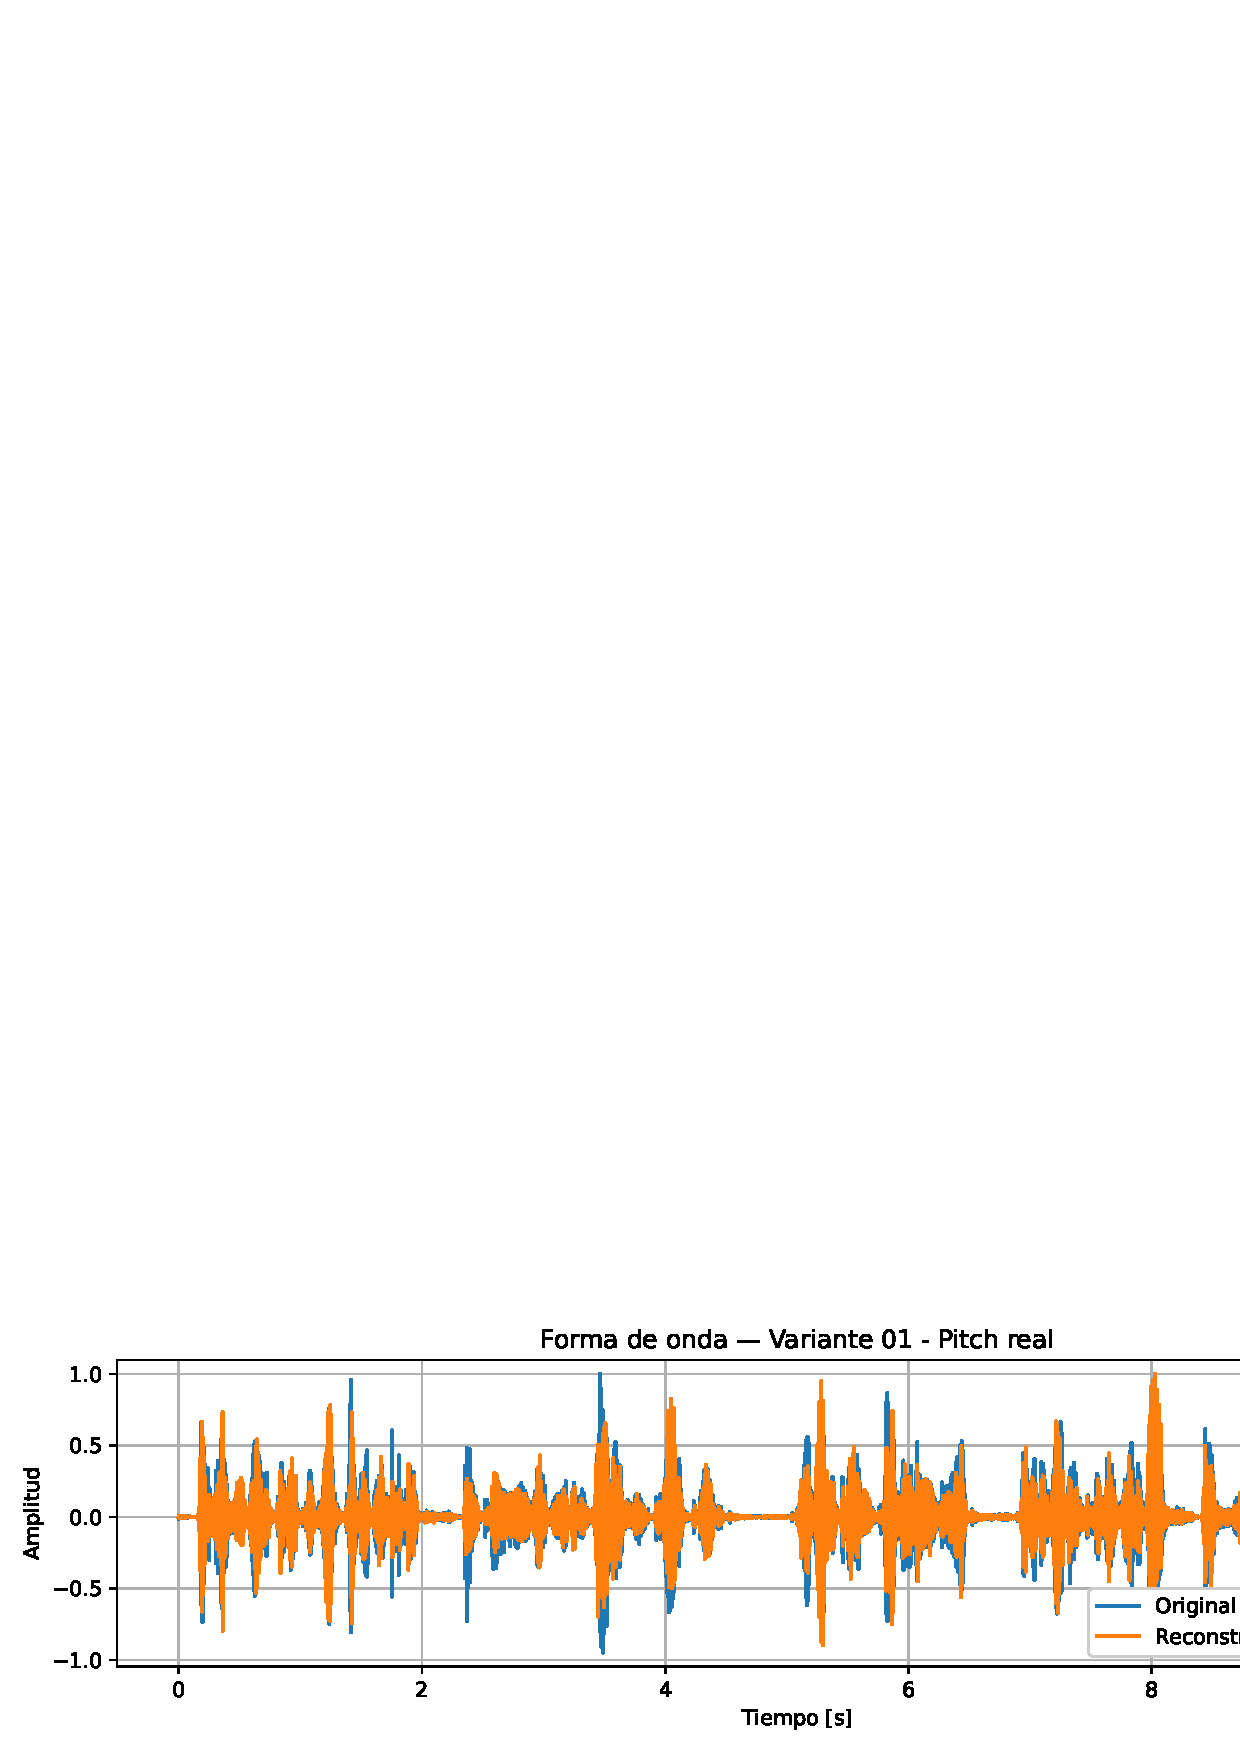
\includegraphics[width=\linewidth]{res/onda_01_a.pdf}
    \caption{Superposición de señal real y reconstruida en el tiempo}
    \label{fig:onda_01_a}
\end{figure}

\begin{figure}[H]
    \centering
    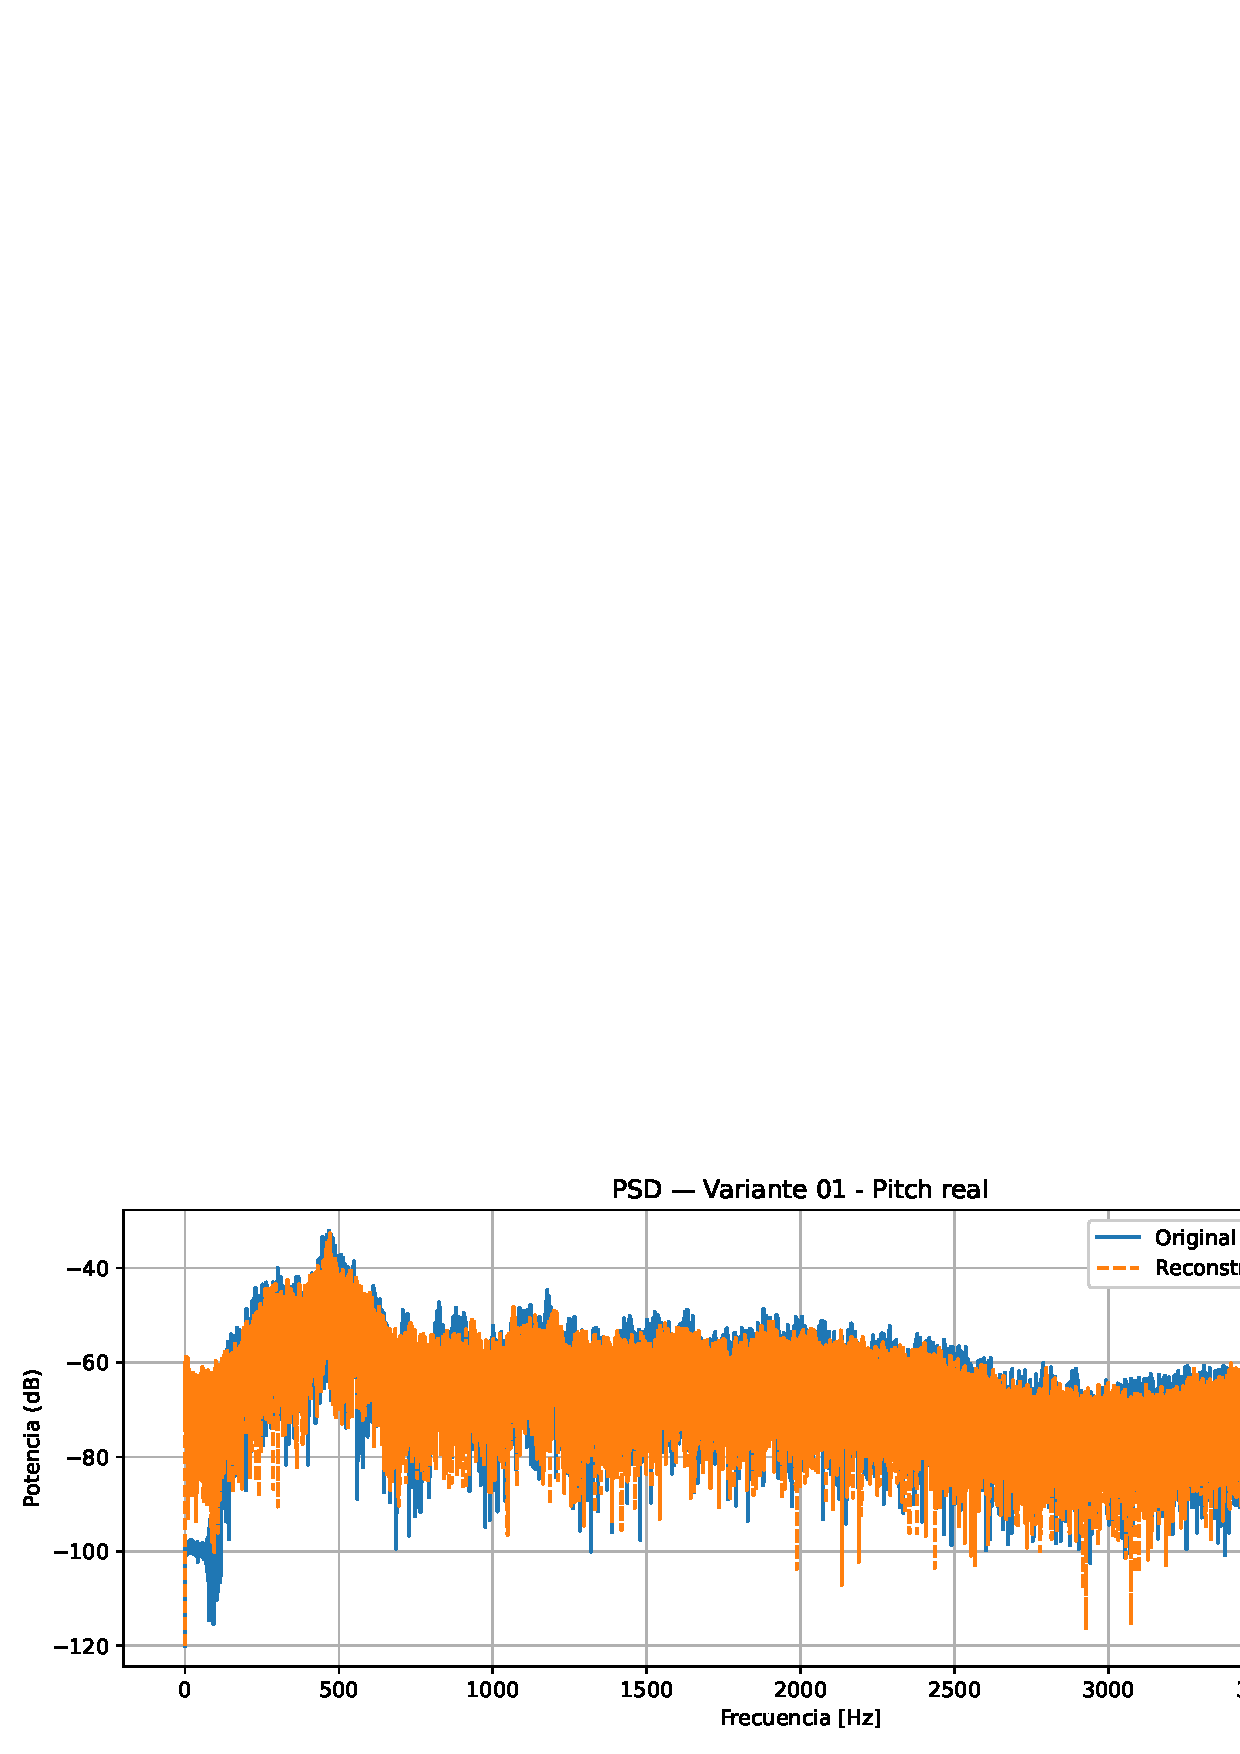
\includegraphics[width=\linewidth]{res/psd_01_a.pdf}
    \caption{Superposición de PSD real y reconstruida}
    \label{fig:psd_01_a}
\end{figure}

\quad En este caso se puede ver que, si bien ni la PSD ni la señal en el tiempo son coincidentes en todos los puntos, en el caso de la señal en el tiempo los máximos de amplitud coinciden, y en la PSD la forma general, ignorando el ruido, es similar.

\quad Escuchando el audio de la señal reconstruida, es posible entender el relato de la persona, si bien el sonido no es idéntico. 

\subsection{Reconstrucción con pitch fijo}

\quad En este caso se utilizó un pitch fijo de \SI{200}{Hz} para todos los fragmentos.

\begin{figure}[H]
    \centering
    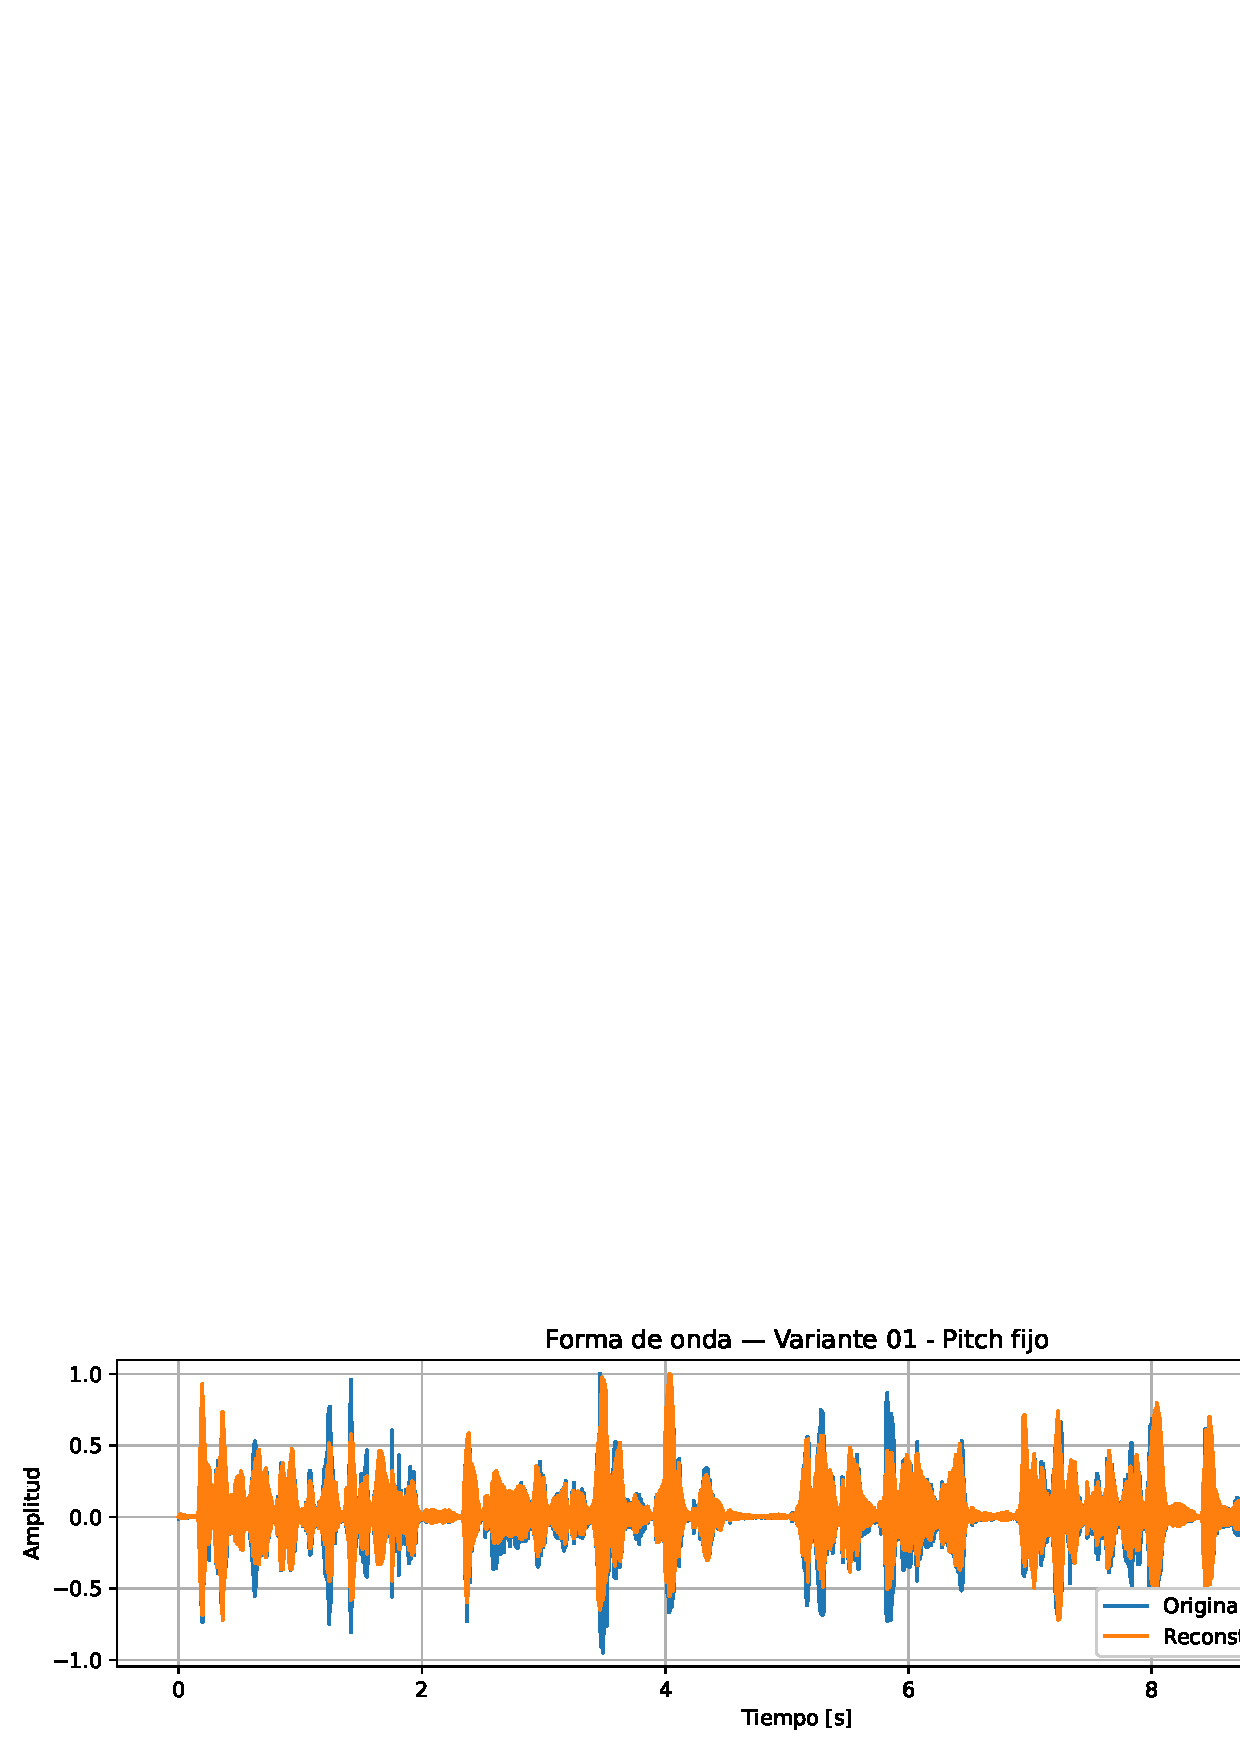
\includegraphics[width=\linewidth]{res/onda_01_b.pdf}
    \caption{Superposición de señal real y reconstruida en el tiempo}
    \label{fig:onda_01_b}
\end{figure}

\begin{figure}[H]
    \centering
    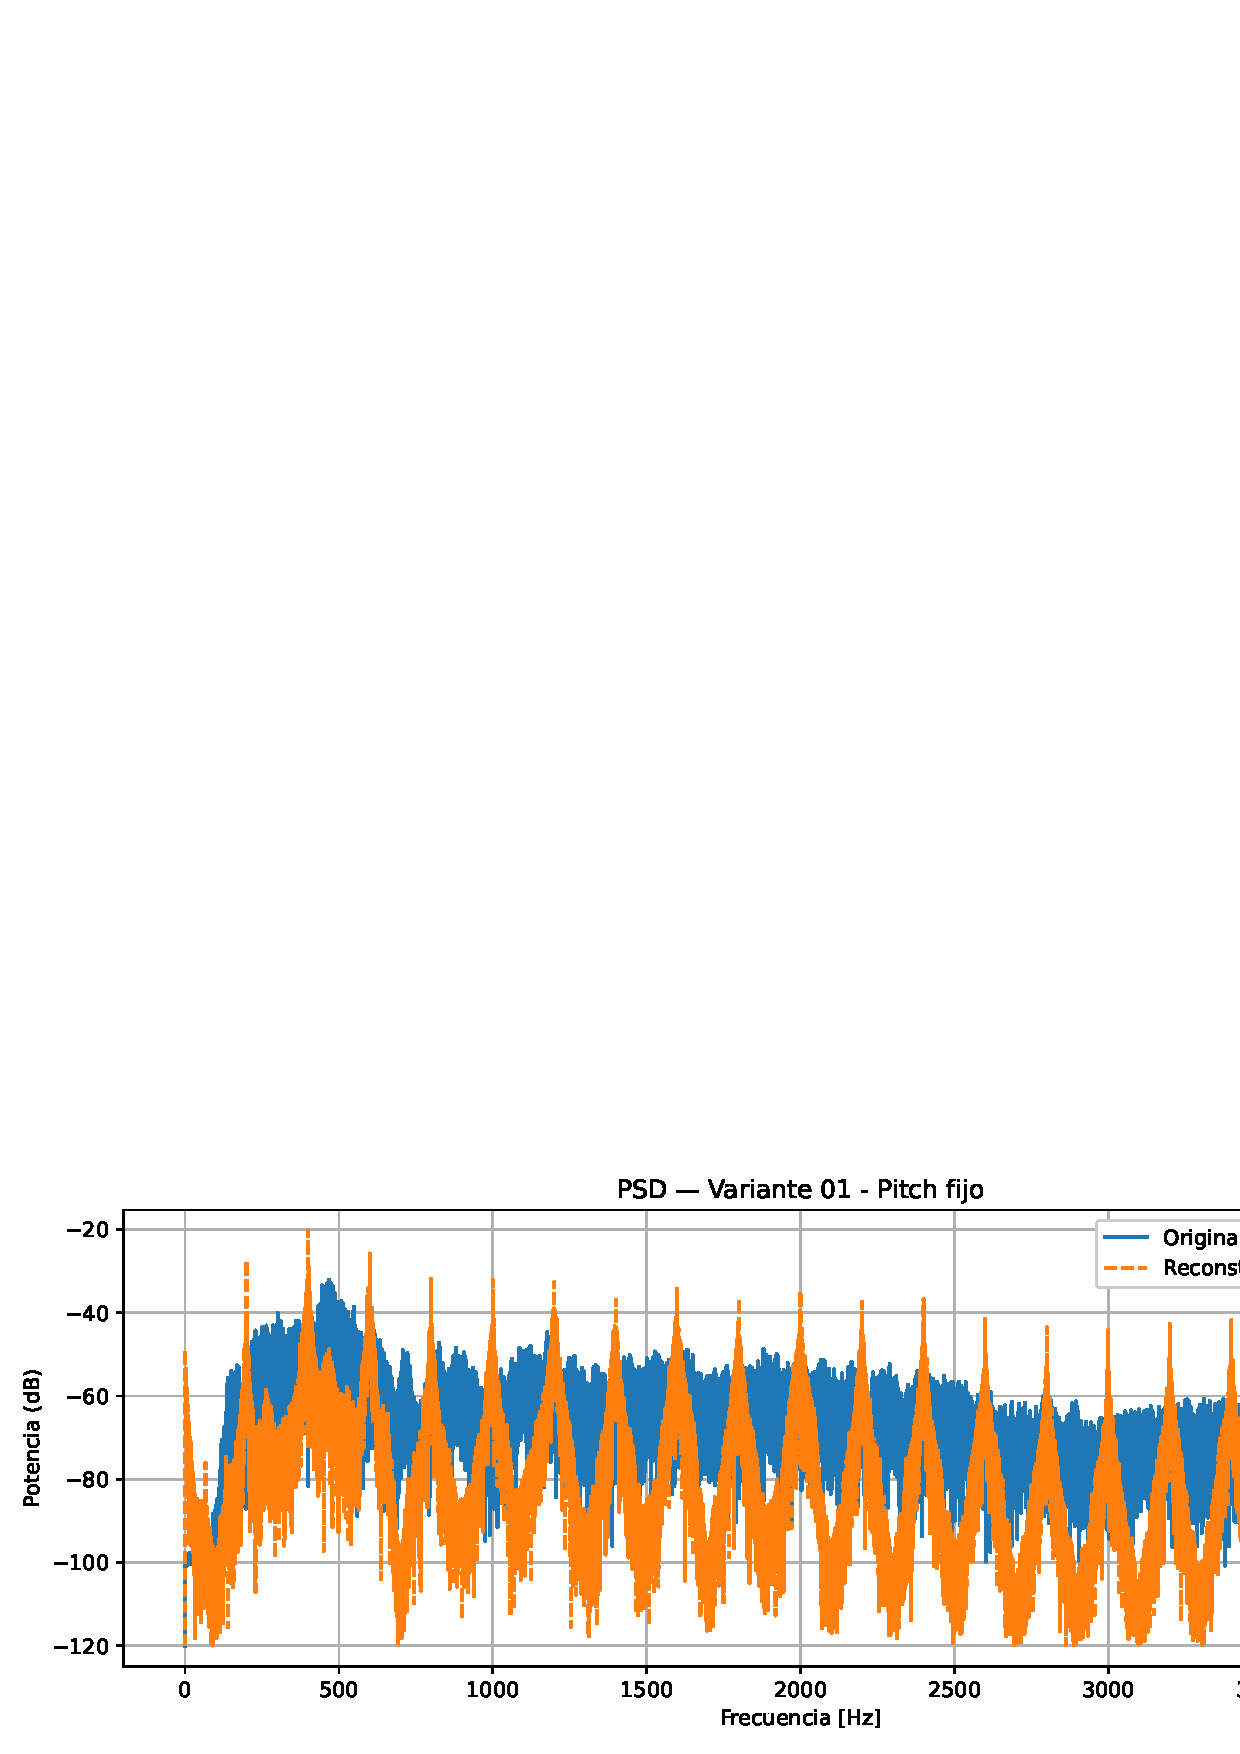
\includegraphics[width=\linewidth]{res/psd_01_b.pdf}
    \caption{Superposición de PSD real y reconstruida}
    \label{fig:psd_01_b}
\end{figure}

\quad En la \autoref{fig:psd_01_b} se puede ver claramente el efecto de usar un pitch fijo, en este caso los gráficos no coinciden en lo absoluto, si bien la forma de onda temporal pueda ser similar. 

\quad Esto resulta en que el audio obtenido mantenga el sonido de la voz diferenciable, pudiendo entender el relato, pero con un sonido \textit{robótico}.

\subsection{Reconstrucción sin pitch}

\quad Ahora en vez de utilizar un pitch para la reconstrucción de los fragmentos, se utiliza ruido blanco en todos los casos.

\begin{figure}[H]
    \centering
    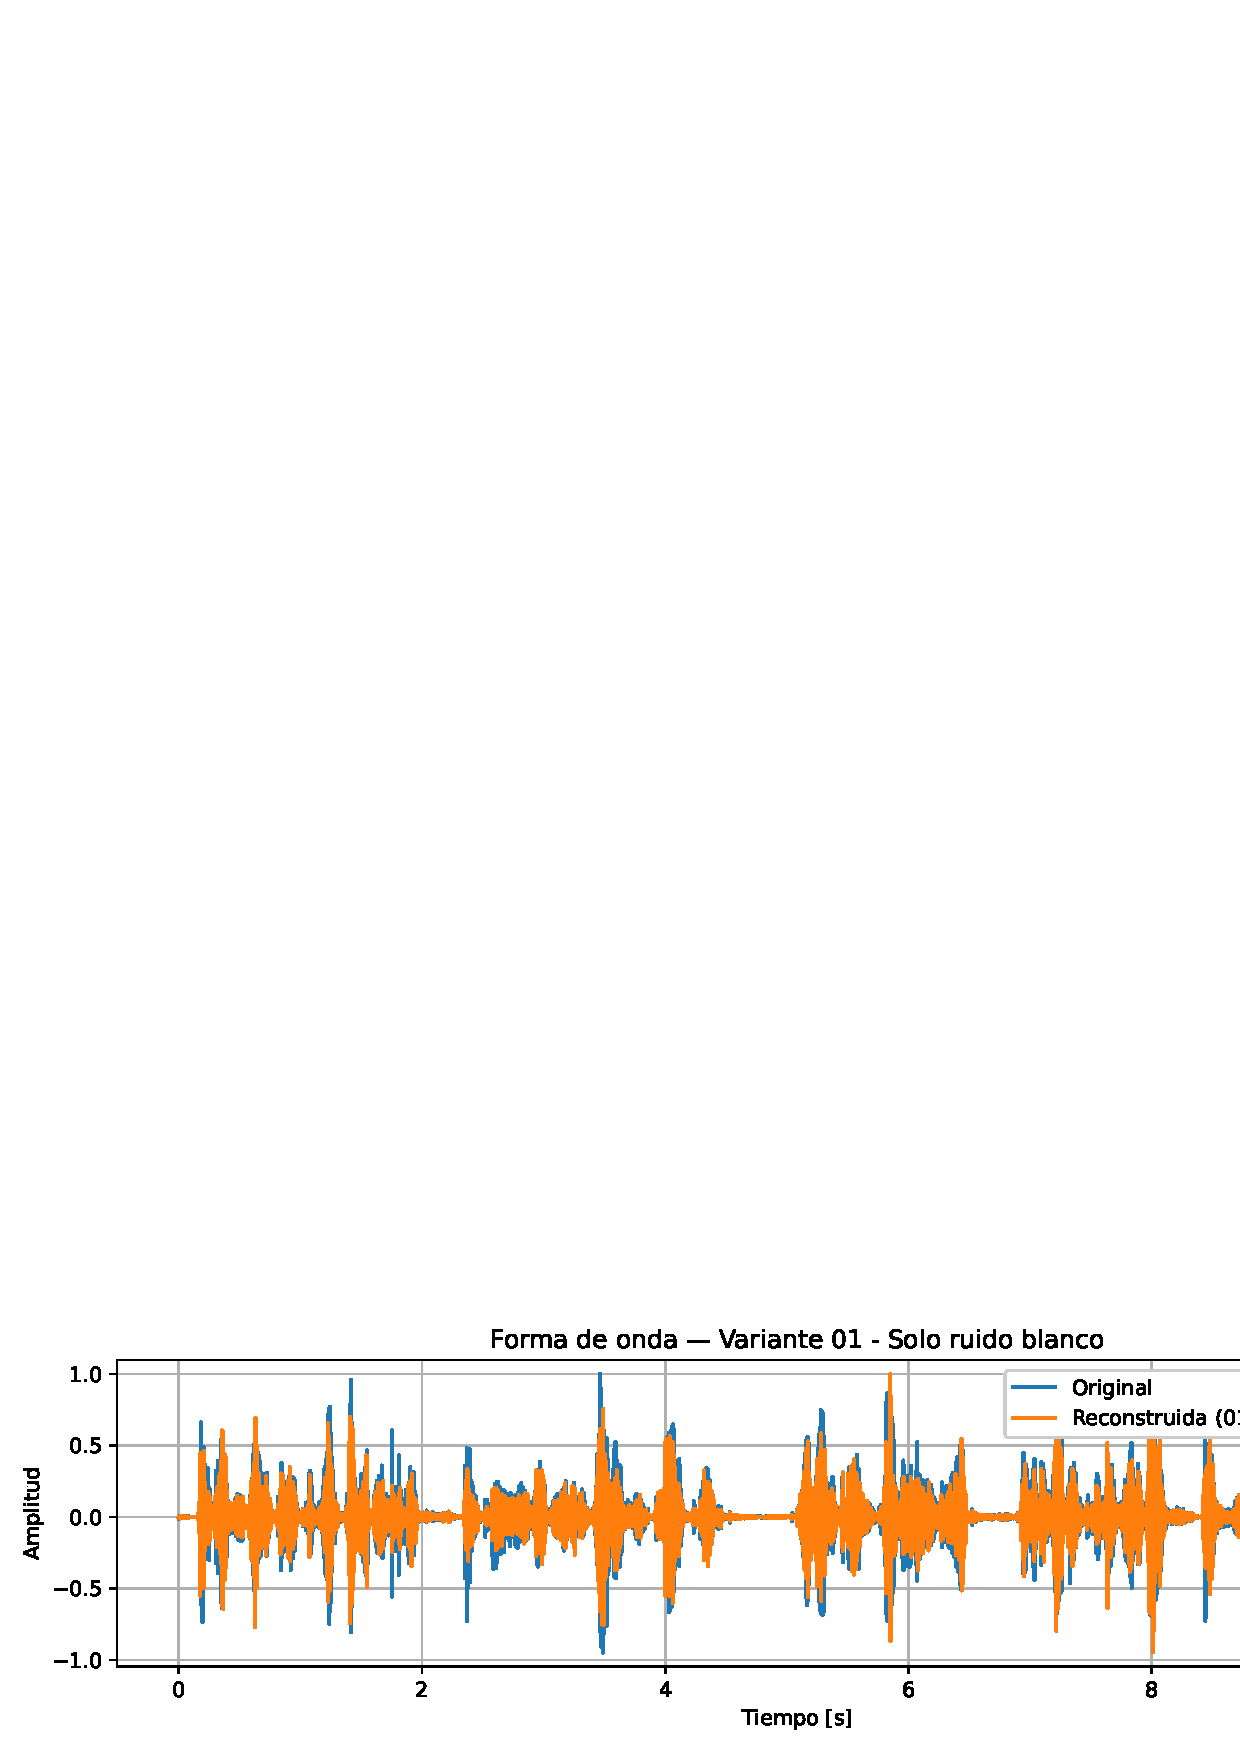
\includegraphics[width=\linewidth]{res/onda_01_c.pdf}
    \caption{Superposición de señal real y reconstruida en el tiempo}
    \label{fig:onda_01_c}
\end{figure}

\begin{figure}[H]
    \centering
    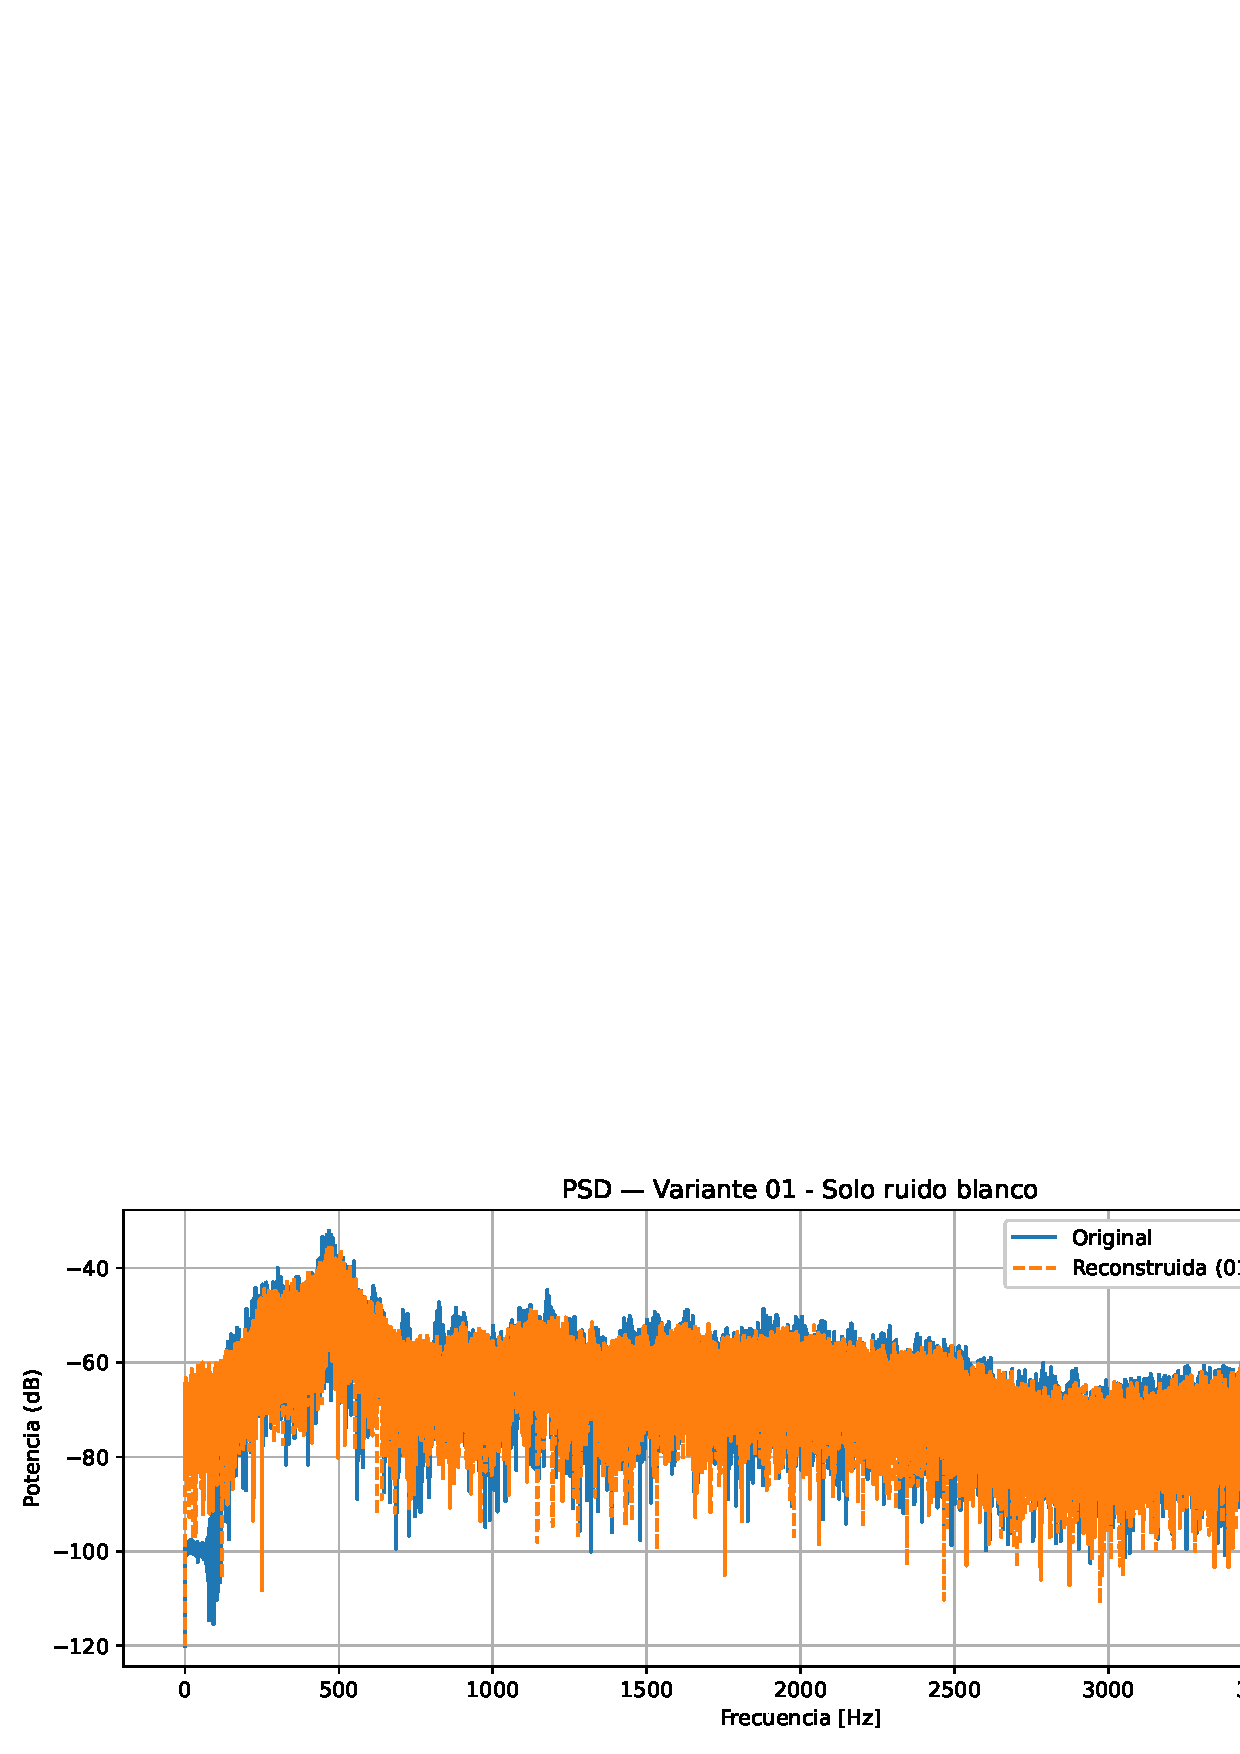
\includegraphics[width=\linewidth]{res/psd_01_c.pdf}
    \caption{Superposición de PSD real y reconstruida}
    \label{fig:psd_01_c}
\end{figure}

\quad En las figuras de este caso se puede ver que no se presenta demasiada diferencia entre el reconstruido y el real. Sin embargo, al escuchar el audio reconstruido se nota una clara diferencia, el no usar pitch y reconstruir la señal solamente con ruido blanco resulta en una voz similar a la que utiliza al susurrar. 

\subsection{Reconstrucción con pitch sintético}

\quad Para este ultimo caso se utilizó un pitch artificial generado por el fragmento de código proporcionado por los docentes.

\begin{figure}[H]
    \centering
    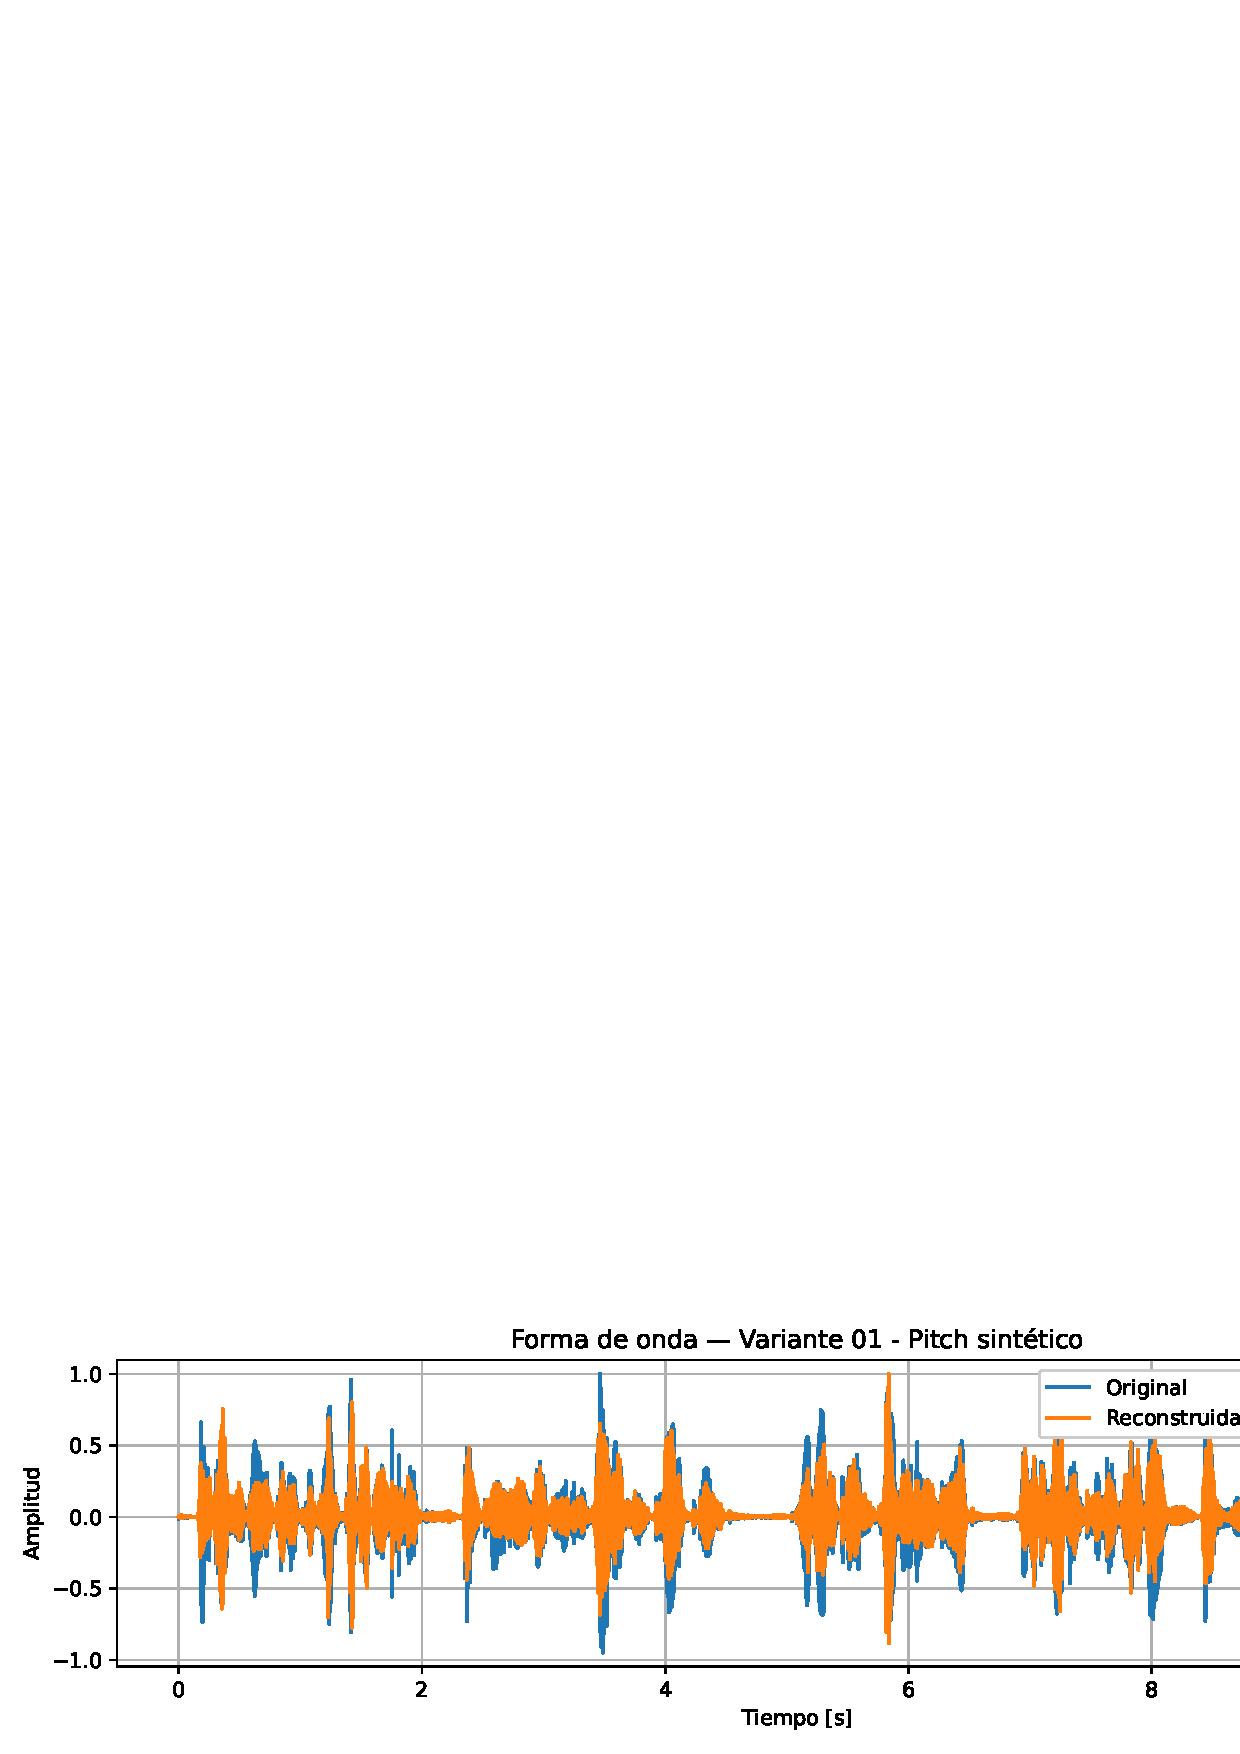
\includegraphics[width=\linewidth]{res/onda_01_d.pdf}
    \caption{Superposición de señal real y reconstruida en el tiempo}
    \label{fig:onda_01_d}
\end{figure}

\begin{figure}[H]
    \centering
    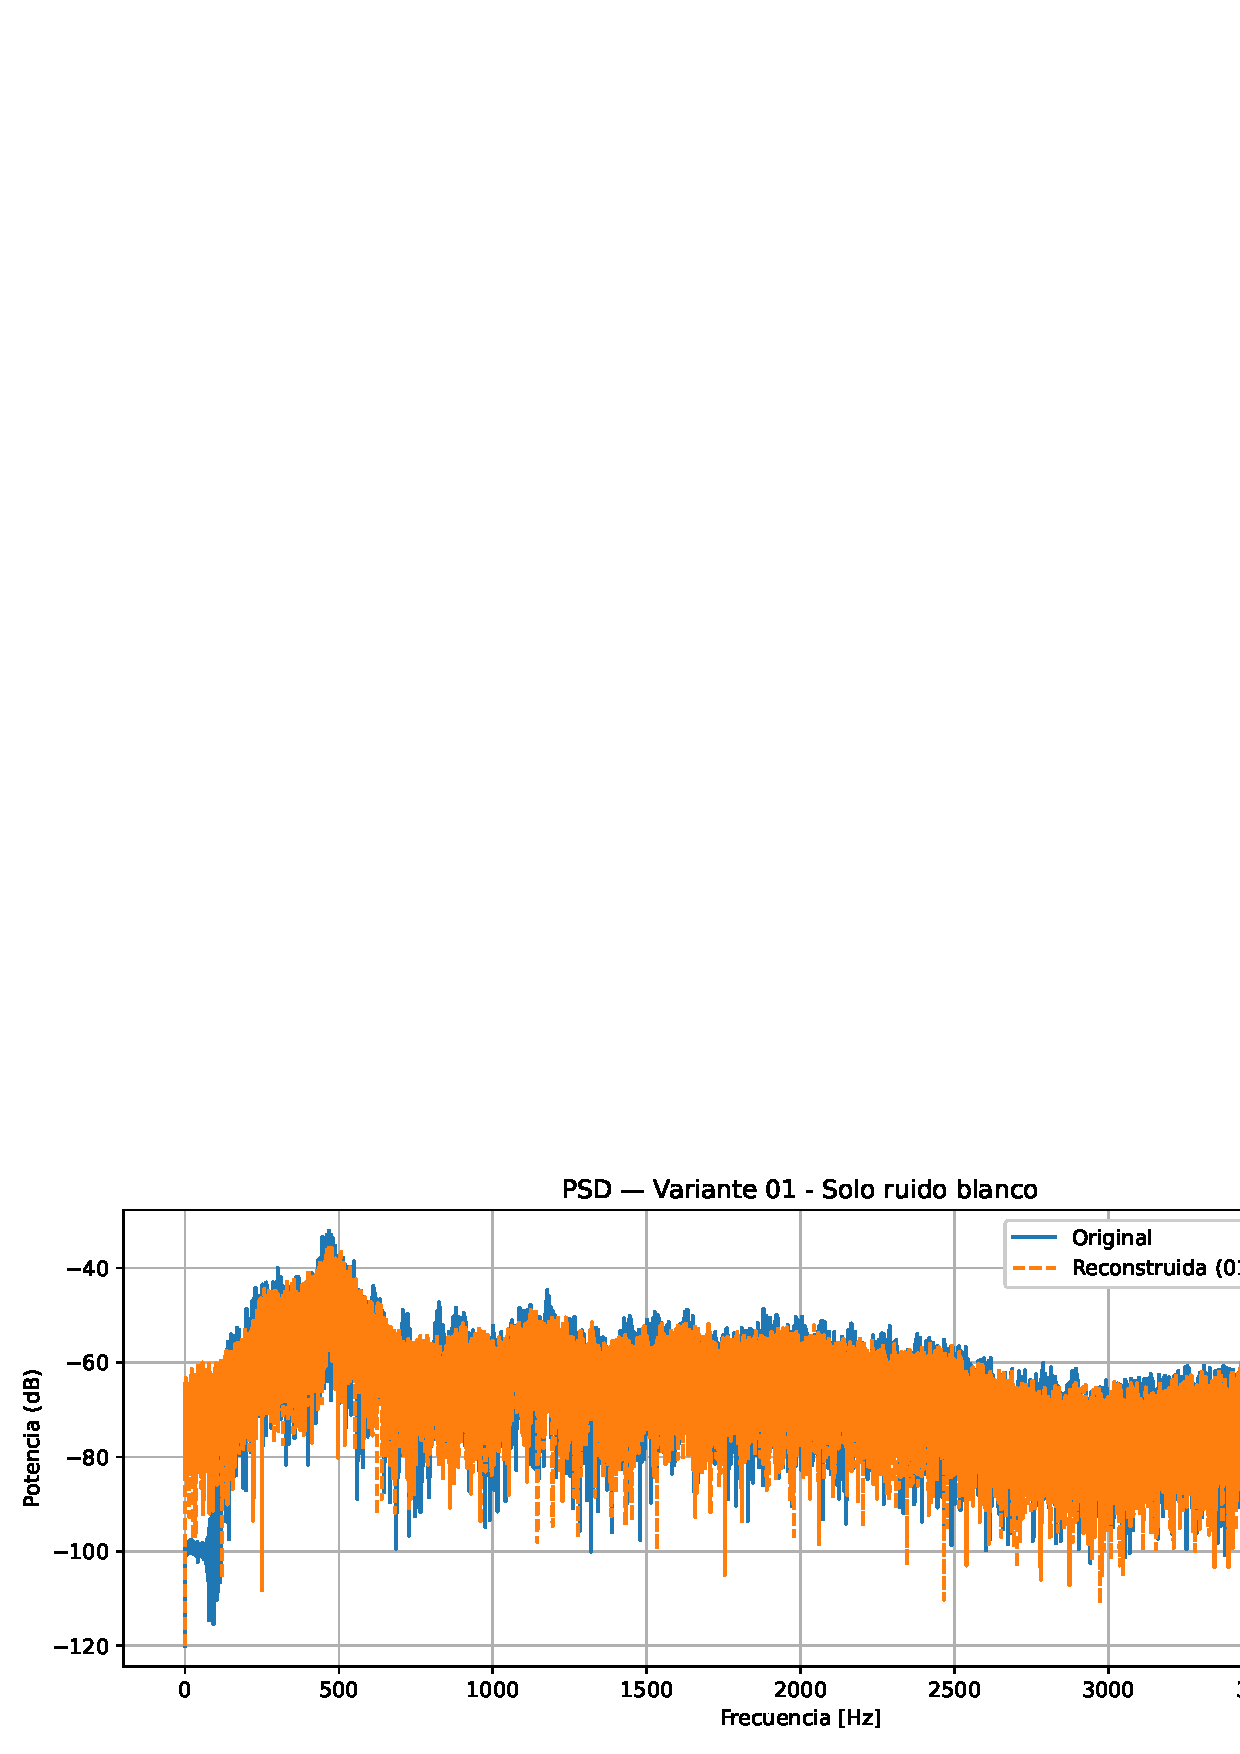
\includegraphics[width=\linewidth]{res/psd_01_c.pdf}
    \caption{Superposición de PSD real y reconstruida}
    \label{fig:psd_01_d}
\end{figure}

\quad Nuevamente en este caso no se presenta amplia diferencia en los gráficos, pero al escuchar el audio reconstruido es posible apreciar el efecto del pitch variable.

\section{Conclusiones}

\quad A pesar de que los audios sintetizados no sean exactamente iguales a los originales, se puede identificar el relato de manera clara en todos los casos. Se observó el efecto de utilizar pitchs obtenidos desde distintas fuentes en los audios. 

\quad Se comprobó que el rango de ventaneo en este tipo de estimación no puede ser tan chico porque es posible que no hayan suficientes periodos muestreados, disminuyendo la resolución espectral.

\quad Comenzando por la obtención de los coeficientes del modelo LPC y estimando el pitch de los fragmentos se pudo codificar audios a través de un ventaneo. Luego con los datos obtenidos se pudieron reconstruir los fragmentos, con suficiente exactitud para entender los relatos en estos.


\end{document}